\chapter{Arquitectura}
\label{Arquitectura}
Este apartado describe la arquitectura software de \textbf{Virus Breaker}. La descripción comenzará con una recapitulación de los eventos con los que un jugador se encontrará cuando inicie una sesión de juego. A esta descripción le seguirá a un análisis técnico de la estructura interna del juego, comenzando por las \textbf{escenas} en las que este se divide y terminando con un análisis de cada uno de los \textbf{objetos} que intervienen en el desarrollo de la acción.

\section{Descripción del Juego}
Como programa informático, Virus Breaker constara de un \textbf{archivo ejecutable}, acompañado de una carpeta que almacena ficheros complementarios. Para iniciar el juego, el jugador deberá simplemente iniciar el archivo ejecutable, sin necesidad de ningún tipo de instalación previa.

Una vez iniciado, el juego presentará al jugador una sencilla \textbf{pantalla de titulo}. La funcionalidad de esta pantalla será limitada, solo mostrará el título y el nombre del desarrollador del juego e informará al jugador de que botón debe pulsar para iniciar una partida. En la figura \ref{titulo} se puede ver la apariencia de esta pantalla de título en la versión final del juego.
\begin{figure}[h]
    \centering
    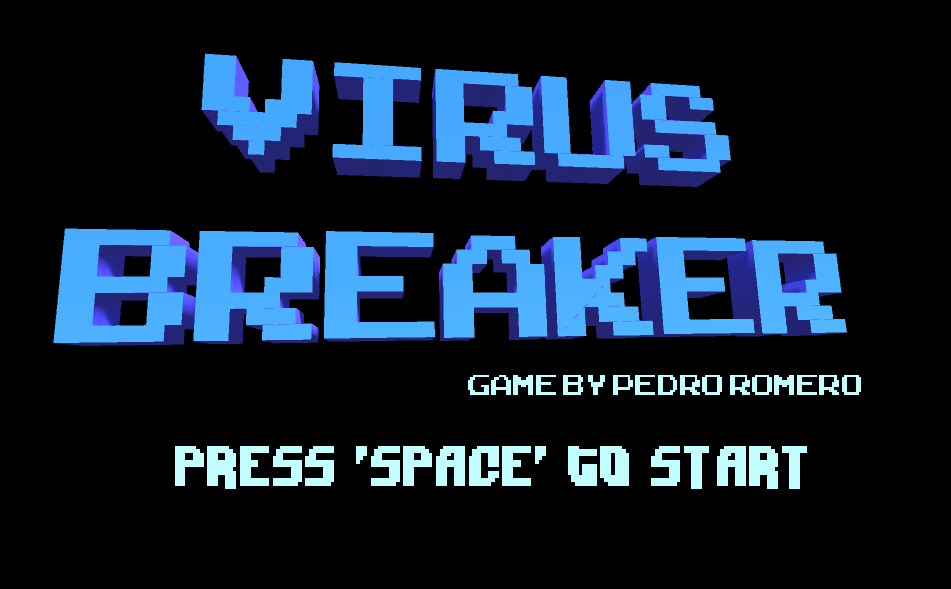
\includegraphics[width=0.6\textwidth]{images/estructura/descripcion/titulo}
    \caption{Pantalla de título.}
    \label{titulo}
\end{figure}

Una vez iniciada la partida, el jugador pasará a controlar al \textbf{personaje principal} e intentará superar los desafíos que le presente el juego. Una versión básica de esta pantalla se puede ver en la figura \ref{juego}. El juego se dividirá en varios \textbf{niveles}, cada vez que el jugador supere uno, el juego le presentará otro de dificultad mayor. Esta secuencia de niveles concluirá con el enfrentamiento contra un \textbf{Jefe Final}. Al derrotar al jefe final, el juego mostrara una \textbf{pantalla de victoria}. Esta pantalla será funcionalmente idéntica a la pantalla de título: mostrará un mensaje y permitirá al jugador volver a jugar al juego si pulsa un botón. 

\begin{figure}[h]
    \centering
    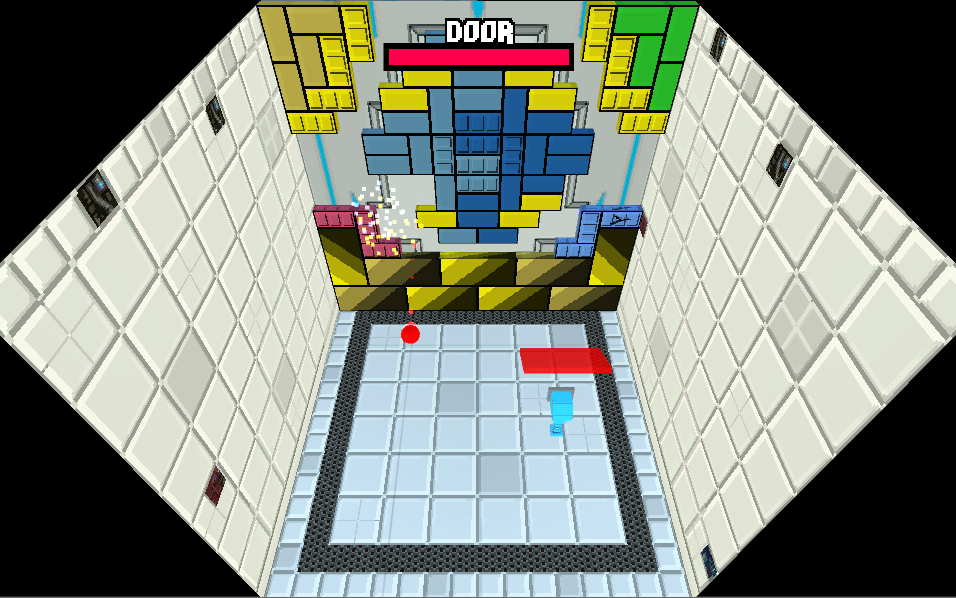
\includegraphics[width=0.6\textwidth]{images/estructura/descripcion/juego}
    \caption{Pantalla de juego.}
    \label{juego}
\end{figure}

Si el jugador es derrotado durante el juego, se le mostrará una pantalla de \textbf{fin del juego}, donde se le ofrecerá la posibilidad de volver a iniciar la partida desde el ultimo nivel superado. A igual que la pantalla de victoria, la funcionalidad de esta pantalla será idéntica a la de la pantalla de título. La similitud entre estas tres pantallas se puede apreciar en la figura \ref{win_lose}.

\begin{figure}[h]
    \centering
    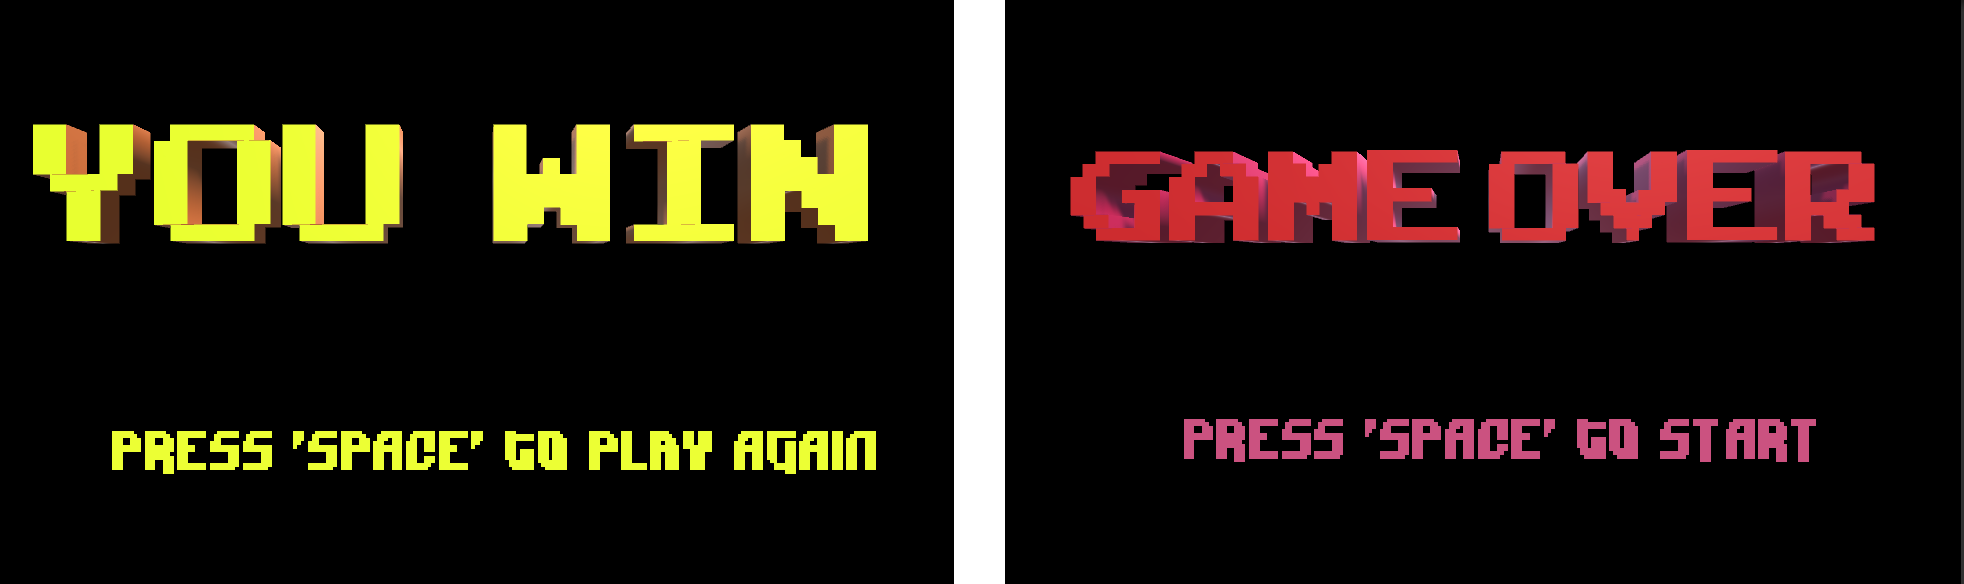
\includegraphics[width=1\textwidth]{images/estructura/descripcion/win_lose}
    \caption{Pantallas de victoria y derrota.}
    \label{win_lose}
\end{figure}

El progreso del jugador en el juego se guarda entre partidas, de forma que, si el juego se cierra, el jugador pueda empezar por el mismo nivel en el que se encontraba la siguiente vez que inicie el juego. Cuando se derrota al jefe final, la partida guardada se elimina para permitir que el jugador pueda volver a jugar desde el principio si lo desea.

\section{Visión general}
La arquitectura de este proyecto está basada en la \textbf{arquitectura de componentes} de Unity, en la que el comportamiento y propiedades de los objetos está determinado por los \textbf{componentes} que estos tengan adheridos. Sin contar con los componentes incluidos de serie en Unity3D, para este proyecto se implementaron \textbf{17 componentes}.

Para implementar los componentes se utilizó el lenguaje de programación \textbf{C\#} al ser el lenguaje más utilizado en el desarrollo con Unity3D. Los componentes desarrollados son \textbf{clases} de C\# que heredan de la clase \textbf{MonoBehaviour}, clase abstracta que implementa la funcionalidad común a todos los componentes. En adición a los componentes, también se implementaron dos \textbf{clases de soporte} adicionales para facilitar el funcionamiento de ciertos componentes.

Las clases elaboradas para el proyecto pueden agruparse en varios \textbf{grupos funcionales} según la función que cumplan en el proyecto. En la figura \ref{diagrama_clases} pueden verse la organización de las clases en sus respectivos grupos.
\begin{figure}[h]
    \centering
    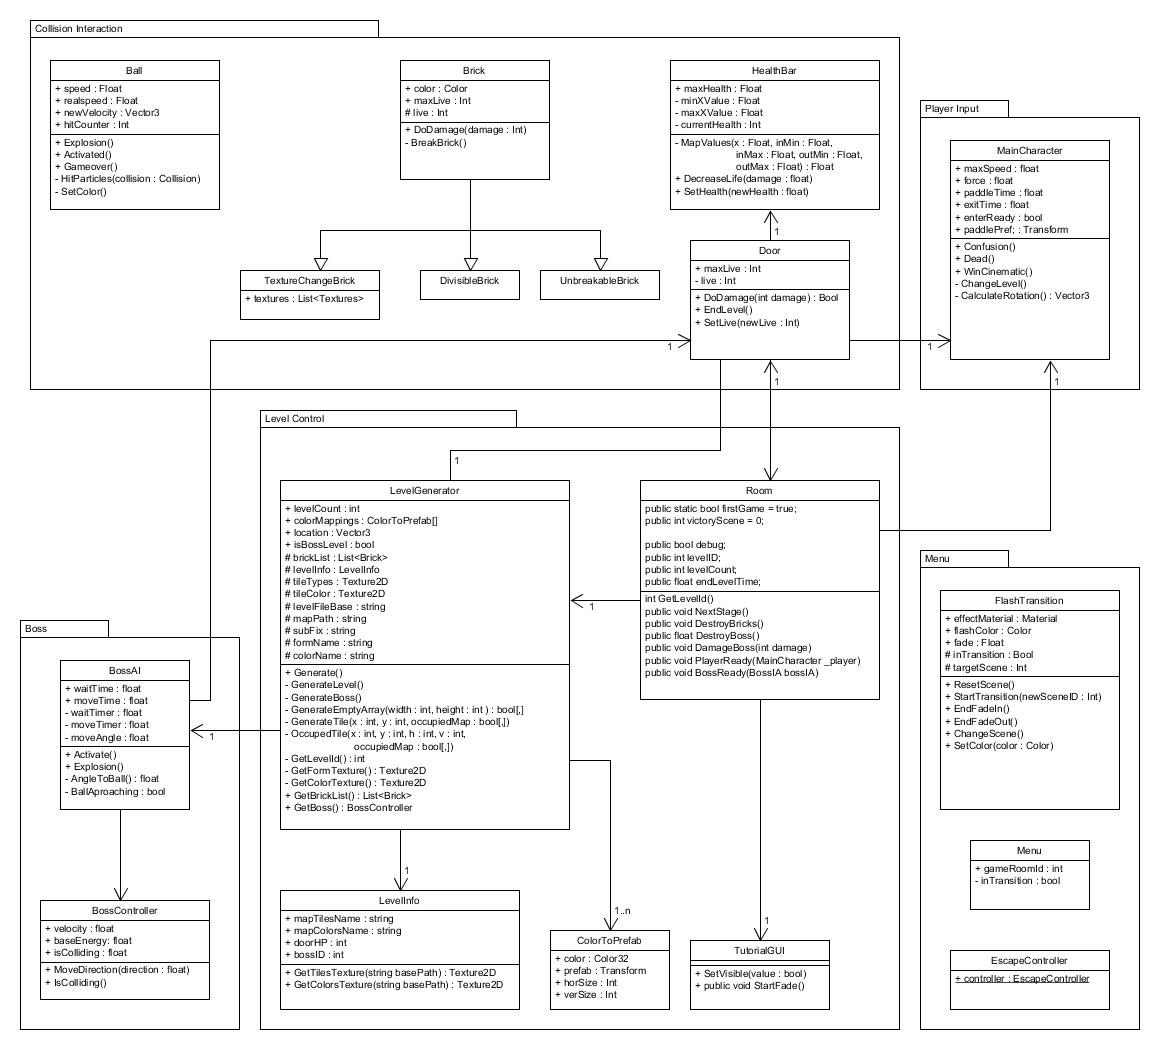
\includegraphics[width=1\textwidth]{images/estructura/vision/diagram}
    \caption{Diagrama de clases.}
    \label{diagrama_clases}
\end{figure}

Los grupos funcionales son los siguientes:
\begin{itemize}
\item \textbf{Menu}: Se trata de clases involucradas la gestión de los menús del juego. La función de estas clases es la de leer la entrada del jugador durante las escenas de menús e iniciar la transición a las escenas pertinentes.
\item \textbf{Level Control}: En este grupo se encuentran las clases implicadas en la correcta ejecución del nivel. El grupo incluye el generador de niveles, que carga la configuración del nivel desde archivo, y los componentes encargados de gestionar que los eventos de la partida se ejecuten en el orden correcto.
\item \textbf{Player Control}: Este grupo incluye una única clase: el comportamiento del jugador. La clase lee la entrada del jugador y ejecuta las acciones correspondientes del personaje principal.
\item \textbf{Collision and Interaction}: En este grupo se encuentra el comportamiento de la pelota y el de los objetos que reaccionan a su colisión.
\item \textbf{Boss Control}: Este grupo contiene las clases que determinan el comportamiento del jefe final del juego.
\end{itemize}

\section{Menú}
Virus Breaker cuenta con cuatro \textbf{Escenas}: La \textbf{escena de juego}, que es donde ocurre toda la acción y tres \textbf{escenas de menú}. Las escenas de menú sirven como intermedio entre sucesivas sesiones de juego y permiten que el jugador se pueda prepararse antes de empezar con el juego.

El comportamiento del juego en estas tres escenas es prácticamente es muy básico: El juego muestra un texto animado de gran tamaño, acompañado de un segundo texto (también animado) con instrucciones para el jugador. Si el jugador pulsa la tecla \textbf{espacio}, la escena cambiará a la escena de juego. Los tres menús son los siguientes:
\begin{itemize}
\item \textbf{La escena de titulo}. Esta escena aparece nada más iniciar el juego. Esta escena muestra el título del juego, el nombre del desarrollador.
\item \textbf{La escena de fin del juego}. Esta escena aparece cuando el jugador pierde durante la partida.
\item \textbf{La escena de fin del juego}. Esta escena aparece cuando el jugador supera todos los niveles del juego.
\end{itemize}
En la figura \ref{diagrama_escenas} se pueden ver las transiciones entre las distintas escenas a modo de diagrama de estados.

\begin{figure}[h]
    \centering
    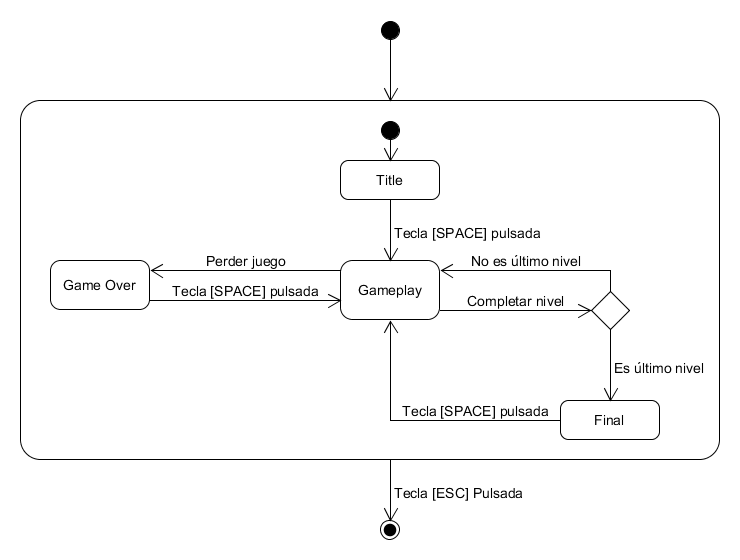
\includegraphics[width=0.8\textwidth]{images/estructura/menu/scenes}
    \caption{Diagrama de escenas.}
    \label{diagrama_escenas}
\end{figure}

La clase que controla el comportamiento de los menús es \textbf{Menu}. Esta clase lee la entrada del jugador durante el método \textbf{Update} a la espera de que este pulse la tecla espacio. Cuando detecta la pulsación, la clase inicia el cambio de escena. Esta clase es un componente asociado al texto que muestra las instrucciones.

El cambio de escena se lleva a cabo mediante la clase \textbf{FlashTransition}. Esta clase es un componente asociado a la cámara de la escena (el objeto encargado de renderizar la escena) que se encarga de producir una transición suave entre dos escenas. La transición se activa el método publico \textbf{StartTransition}, a través del cual el componente recibe la escena de destino. El componente aplica un fundido en negro a la escena para a continuación cargar la escena de destino mediante el \textbf{SceneManager} el gestor de escenas de Unity. En la escena destino, una cámara idéntica produce el efecto a la inversa.

El fundido en negro se implementa aplicando una textura semitransparente sobre la imagen capturada por la cámara, cuyo grado de transparencia cambia con el tiempo gracias a un componente \textbf{Animator}. En la figura \ref{camara_components} puede verse la configuración de componentes de la cámara.
\begin{figure}[h]
    \centering
    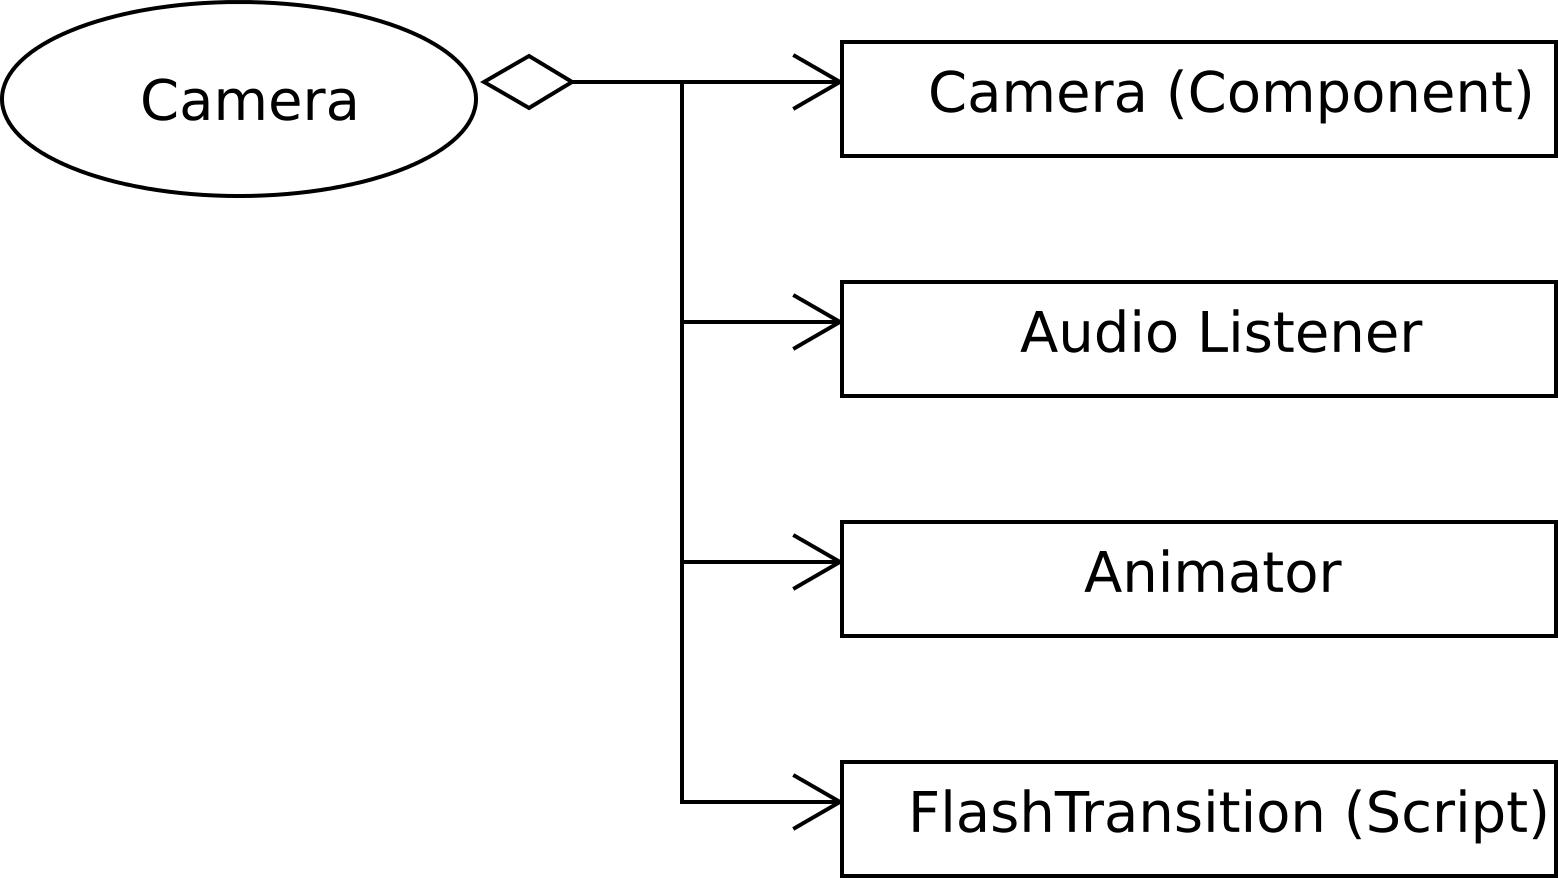
\includegraphics[width=0.6\textwidth]{images/estructura/menu/camera}
    \caption{Componentes de la cámara.}
    \label{camara_components}
\end{figure}

Para la animación de los textos también se utilizó un componente Animator que variaba con el tiempo el ángulo y tamaño de estos. Los textos pequeños fueron creados mediante el sistema de interfaz gráfica de usuario de Unity, pero los textos grandes fueron modelados en \textbf{Blender}\footnote{https://www.blender.org/} y luego importados en Unity.

Adicionalmente al controlador de menús se encuentra la clase \textbf{EscapeController}. Esta clase permite al jugador cerrar el juego en cualquier momento pulsando la tecla \textbf{escape}. La clase es un componente asociado a un objeto vació en la \textbf{escena de titulo} el cual persiste entre escenas gracias al método de Unity \textbf{DontDestroyOnLoad}. Para evitar que varias instancias de este controlador estén presentes, lo que podría provocar errores, se utiliza el patrón de diseño \textbf{Singleton}.

\section{Control de niveles}
La acción del juego ocurre principalmente en la \textbf{escena de juego}. Esta escena contiene la \textbf{sala}, el escenario donde tiene lugar el juego, así como los diversos objetos que forman el juego como el personaje principal o la pelota. Aunque la mayor parte de la acción viene dada por la interacción de los objetos contenidos en la sala, la propia sala también tiene su propio comportamiento, indispensable para la ejecución correcta del juego.

Esta sala es un conjunto de GameObjects agrupados de forma jerárquica (figura \ref{diagrama_sala}), de forma que los diferentes objetos que la conforman tienen una funcionalidad distinta. Los GameObjects son:
\begin{itemize}
\item \textbf{Room}: Es el objeto principal o ``padre'' que contiene a los demás. Contiene tres componentes: un \textbf{Audio Source}, el script \textbf{LevelGenerator} y el script \textbf{Room}.
\item \textbf{Walls}: Se trata de cuatro rectángulos que forman las tres paredes de la sala y el techo (que es funcionalmente idéntico a las paredes). Estos GameObjets tienen dos componentes: Un \textbf{MeshCollider} y un \textbf{Renderer}.
\item \textbf{Floor}: El suelo de la sala es similar a las paredes (un GameObject con un \textbf{MeshCollider} y un \textbf{Renderer}), pero está marcado de forma diferente para activar un comportamiento distinto en la pelota.
\item \textbf{Door}: La puerta de la sala ocupa la pared norte de la sala. 
\end{itemize}

\begin{figure}[h]
	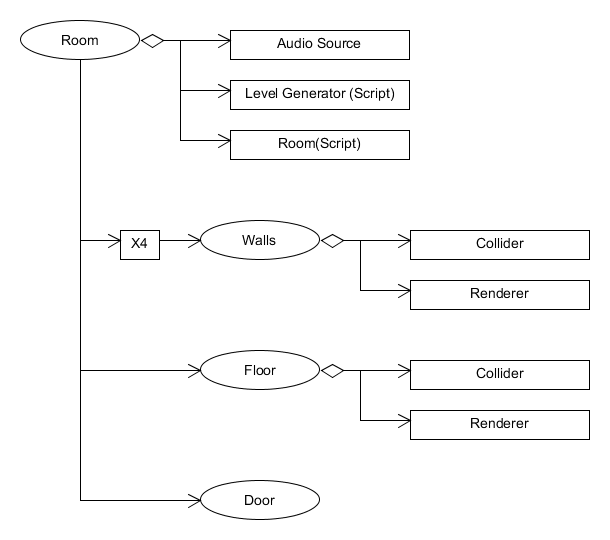
\includegraphics[width=0.8\textwidth]{images/estructura/niveles/room}
	\centering
	\caption{Diagrama de componentes de la sala.}
	\label{diagrama_sala}
\end{figure}

La función principal de la sala es la de gestionar la ejecución del resto de objetos, de forma que su inicialización y destrucción se ejecuten de forma correcta y sin solapamiento. Gracias a la sala, la ejecución de la escena del juego se divide en cuatro etapas bien diferenciadas:
\begin{itemize}
\item \textbf{Carga del nivel}: La configuración del nivel actual es cargada desde archivo y aplicada a la sala.
\item \textbf{Introducción}: Los objetos de la sala realizan su inicialización.
\item \textbf{Juego}: El jugador toma el control del personaje principal.
\item \textbf{Fin del juego}: Los objetos realizan su finalización. Esta etapa puede tener dos variantes: la \textbf{victoria}, en la que el jugador supera el nivel y pasa al nivel siguiente y la \textbf{Derrota}, en la que el jugador pierde y es enviado a la escena de fin del juego.
\end{itemize}

\subsection{Carga de Niveles}
La primera etapa de la ejecución de la escena de juego es la carga del nivel. En esta etapa, la escena, a través de su componente \textbf{LevelGenerator} accede a una serie de archivos que contienen la configuración del nivel. El componente se encarga de leer dicha información y usarla para generar los ladrillos del nivel en su configuración correcta, asignar los puntos de vida a la puerta del juego e iniciar el jefe final en caso de que se tratase de un nivel de jefe.

\subsubsection{Implementación}
La información de un nivel del juego se encuentra almacenada en forma de tres archivos: un fichero \textbf{JSON} y dos \textbf{imágenes .PNG} de 16X16 pixeles. Las imágenes PNG codifican propiedades de los ladrillos en la sala en sus pixeles, los cuales representan las posibles posiciones en las que un ladrillo puede estar colocado sobre la puerta de la sala. La primera de las imágenes determina a través del color de sus pixeles el tipo de ladrillo que debe colocarse en cada posición de la puerta, mientras que la segunda imagen determina el color del ladrillo colocado en dicha posición.
El archivo JSON, por otro lado, contiene la información adicional del nivel, puntos de vida y si se trata de un jefe, y la dirección a las dos imágenes. 

La lógica para la carga de niveles se encuentra en el componente \textbf{LevelGenerator} de la sala. Este componente tiene como atributos la información necesaria para la carga de nivel como índice del nivel actual, formato del nombre de los archivos, la ruta a la carpeta de donde se guardan los archivos o coordenadas del punto de aparición. 

El componente contiene una lista de objetos de la clase \textbf{ColorToPrefab} que sirve para relacionar cada posible color con un tipo de ladrillos. La clase ColorToPrefab es muy sencilla, estando formada por cuatro atributos: el color, el objeto prefabricado y dos enteros que determinan la longitud del prefabricado. En la figura \ref{prefab_color} se pueden ver la lista de todos los ladrillos prefabricados junto a sus colores correspondientes.
\begin{figure}[h]
	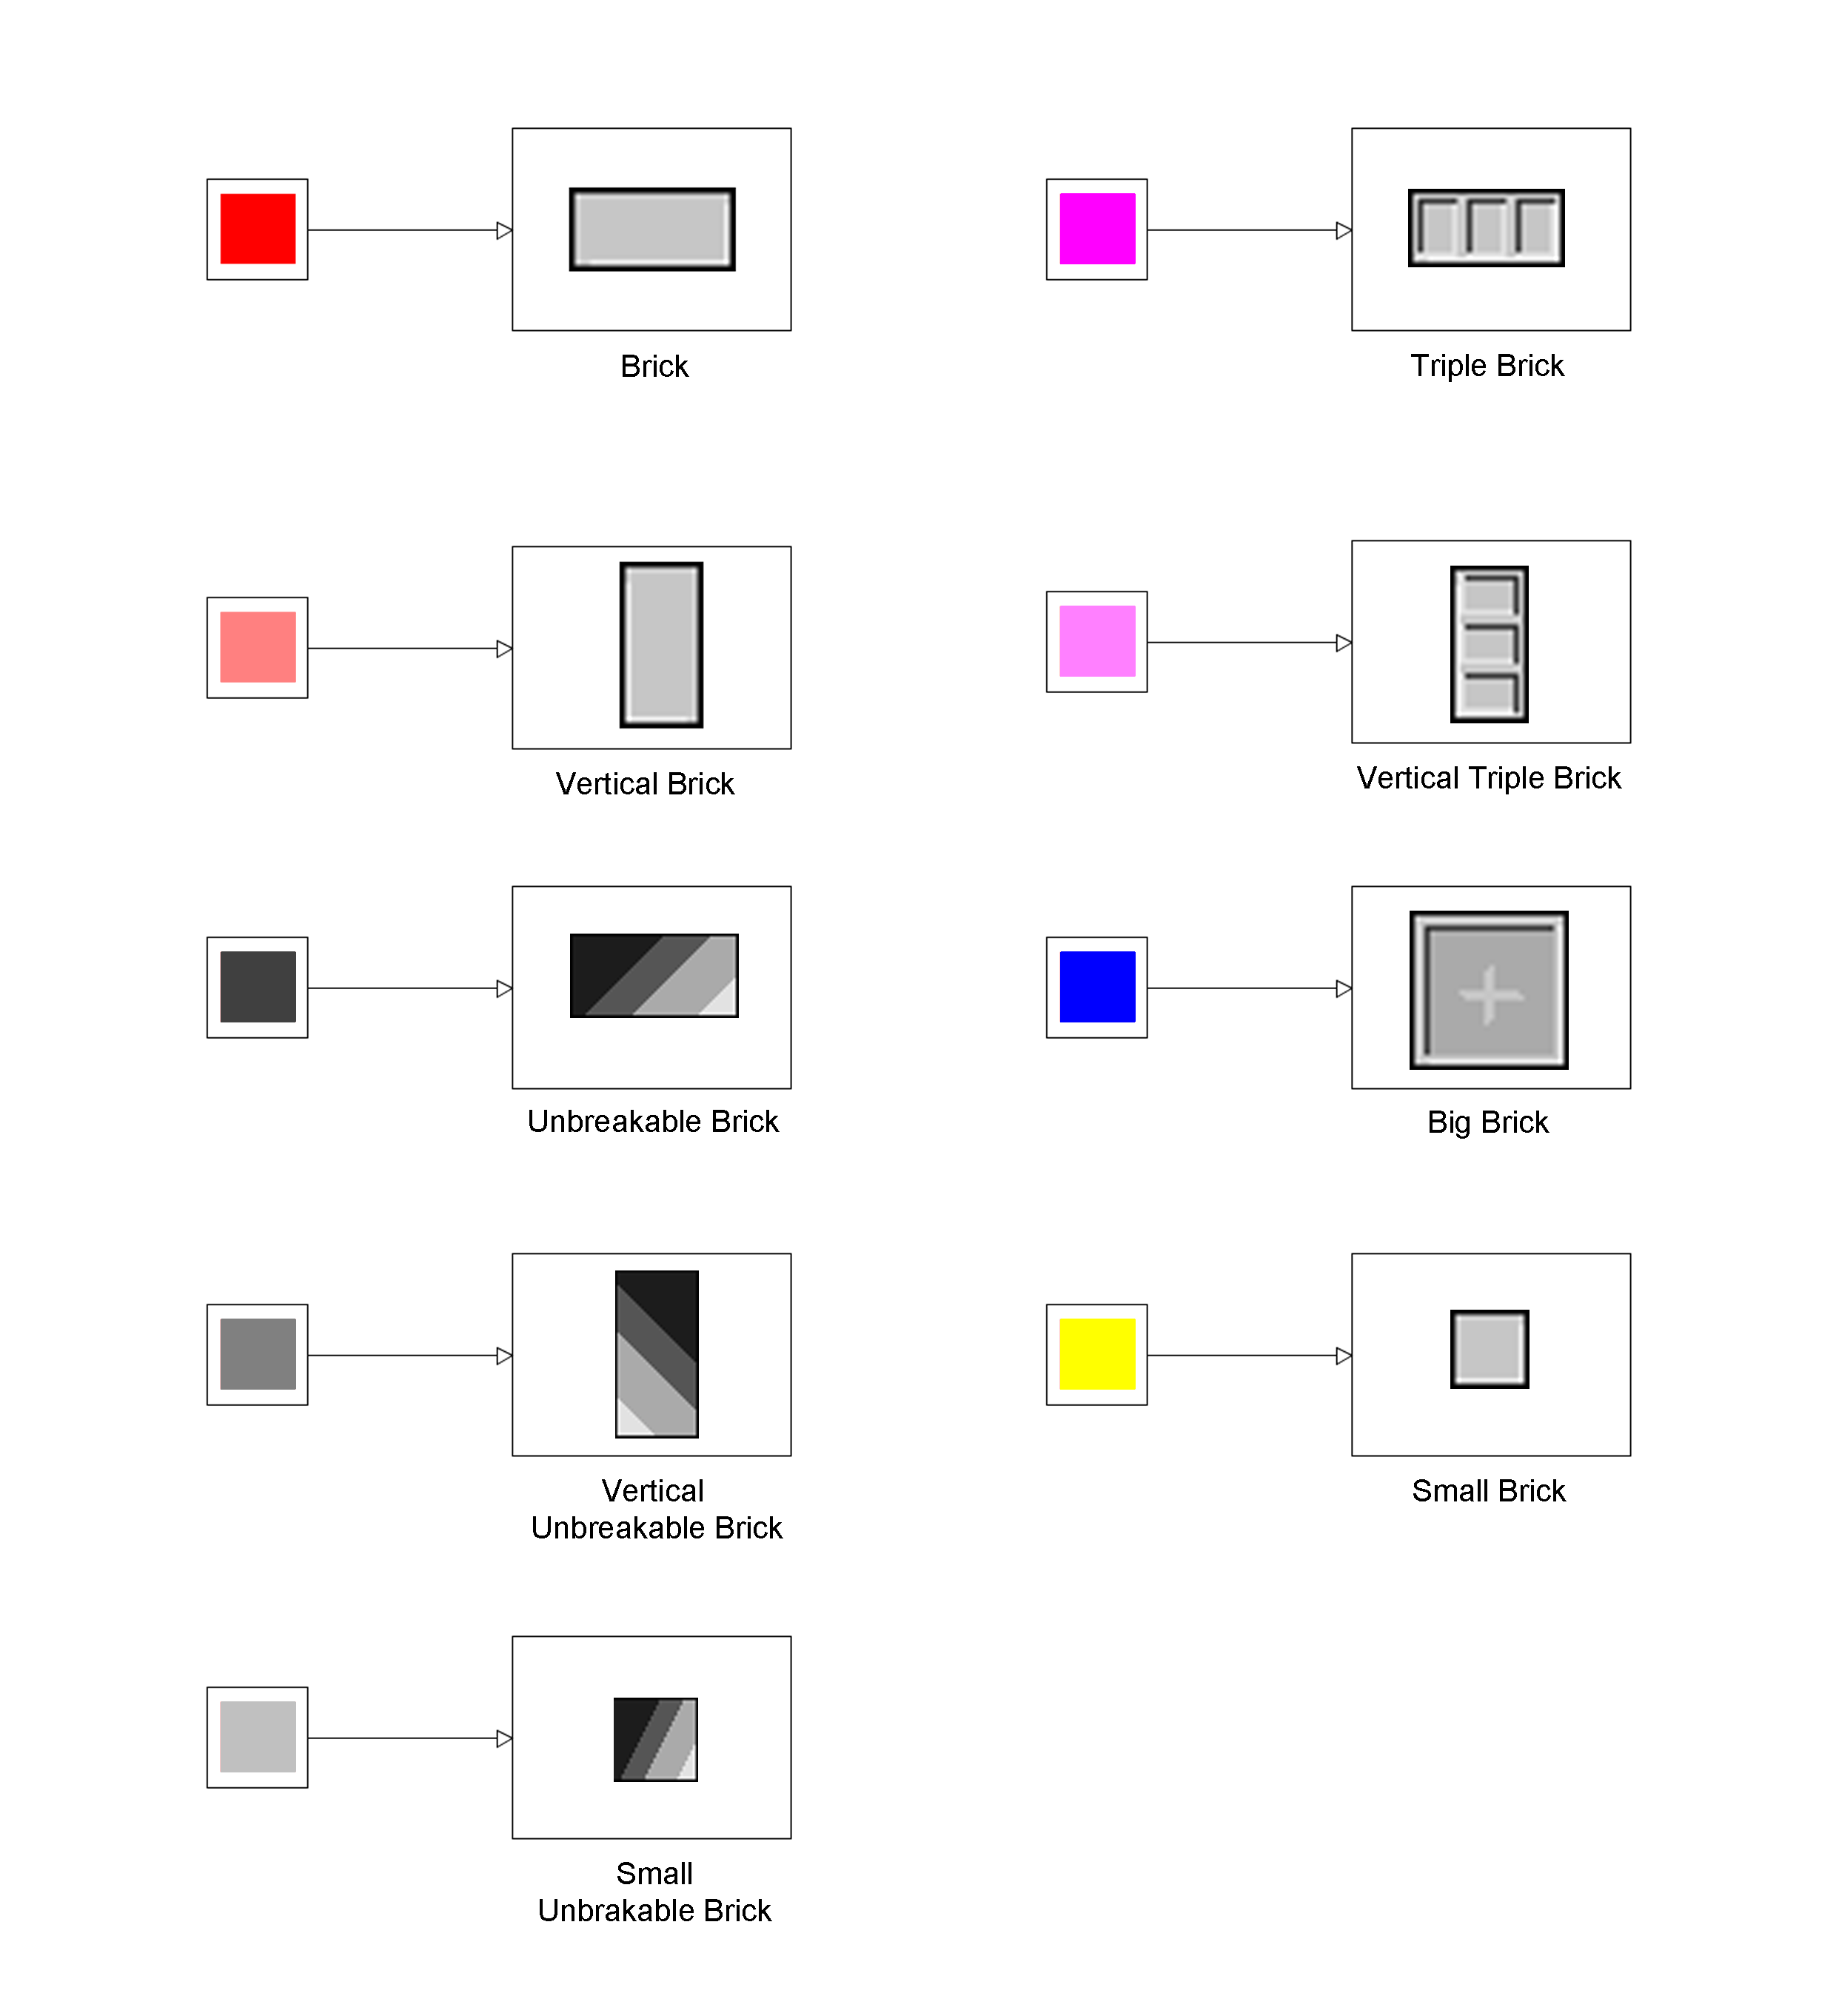
\includegraphics[width=0.8\textwidth]{images/estructura/niveles/prefab_colors}
	\centering
	\caption{Listado de ladrillos prefabricados y sus colores asociados.}
	\label{prefab_color}
\end{figure}


Para iniciar la carga del nivel se utiliza el método público \textbf{Generate} de la clase. El método sigue el siguiente procedimiento para realizar la carga del nivel:
\begin{enumerate}
  \item El componente \textbf{lee archivo JSON} determinado por el índice del nivel actual utilizando la clase \textbf{Resources}\footnote{https://docs.unity3d.com/ScriptReference/Resources.html} de Unity, que permite acceder a assets guardados en una carpeta especial del proyecto. 
  \item Usando la clase JsonUtility\footnote{https://docs.unity3d.com/ScriptReference/JsonUtility.html} de Unity, la información del archivo es convertida en un objeto de la clase \textbf{LevelInfo} lo que facilita su manipulación.
  \item Se \textbf{determina si se trata de un nivel de jefe} o no. En caso afirmativo, se detiene el proceso y se empieza a preparar la batalla con el jefe. En caso contrario, se continua con el proceso.
  \item Se cargan \textbf{las imágenes del nivel} en forma de dos texturas de la clase Texture2D. A efectos prácticos, cada textura es una matriz bidimensional de objetos de clase Color. 
  \item Se instancia una \textbf{matriz de ocupación}, una matriz bidimensional booleana con las mismas dimensiones que las texturas, la cual sirve para marcar que porciones de la puerta están cubiertas por ladrillos.
  \item Se recorre la primera textura \textbf{obteniendo los colores de sus pixeles}. Si la posición correspondiente en la matriz de ocupación está inactiva se realizan las siguientes acciones:
  \begin{enumerate}
  \item El color seleccionado se compara con todos los elementos de la lista de objetos \textbf{ColorToPrefab}. Si alguno de los ColorToPrefab contiene el color seleccionado, se instancia un ladrillo del tipo determinado. Si no hay coincidencia, se pasa al siguiente pixel.
  \item Se accede al color del pixel de la posición actual de la segunda textura. Este color se asigna al ladrillo.
  \item Se marca la posición del ladrillo en la matriz de ocupación. Dado que los ladrillos pueden ocupar más de una ``casilla'', se marcan también las casillas colindantes basándose en los tamaños almacenados en el objeto \textbf{ColorToPrefab}.
  \end{enumerate}
  \item Se asigna \textbf{el número de golpes} que requiere la puerta.
\end{enumerate}
En la figura \ref{generator_diagram} pueden verse de forma gráfica los pasos de ejecución del método
\begin{figure}[h]
	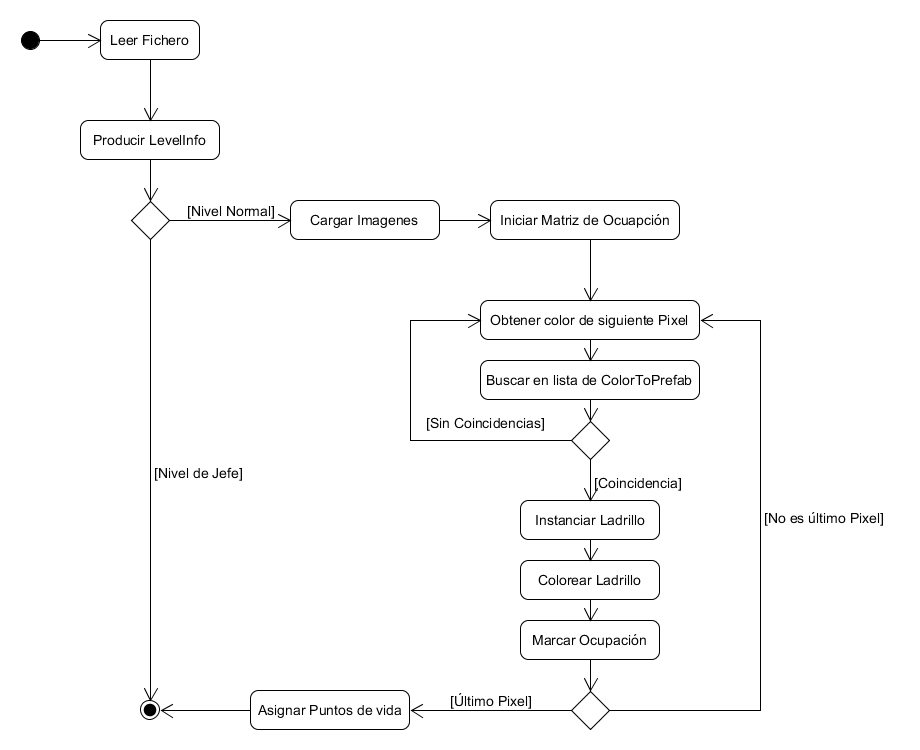
\includegraphics[width=0.8\textwidth]{images/estructura/niveles/level-generator}
	\centering
	\caption{Diagrama del proceso de generación de niveles}
	\label{generator_diagram}
\end{figure}

\subsubsection{desarrollo}
El uso de una única escena de juego con un sistema de carga de nivel se eligió por encima del uso de varias escenas con diferentes configuraciones debido principalmente al gran número de elementos comunes que existen entre los distintos niveles (la geometría de la sala, el personaje, la pelota, la puerta...). De haberse optado por utilizar múltiples escenas, la repetición de elementos \textbf{supondría un gasto innecesario de recursos} y generaría problemas a la hora de realizar \textbf{modificaciones sobre los elementos comunes}, cuyos cambios tendrían que propagarse manualmente en todos los niveles.

Para paliar con estos problemas, se optó por utilizar un editor externo para producir los niveles. Los niveles se \textbf{almacenarían en forma de archivos} que la escena se encargaría de leer para generar las formaciones de ladrillos correspondientes. La funcionalidad que se necesitaba para el editor de niveles era la siguiente:
\begin{itemize}
  \item \textbf{Precisión} a la hora de colocar y alinear los bloques. El editor debe ser capaz de posicionar los ladrillos en una cuadricula de forma automática (para así mantener la estética de juego deseada).
  \item Posibilidad de elegir individualmente el \textbf{color} para cada uno de los bloques del nivel, independientemente de su comportamiento o posición. Esto permite crear dibujos con los bloques, lo que hace los niveles más memorables (ejemplo en la figura \ref{ejemplo-arkanoid}). 
  \item \textbf{Simplicidad} en el proceso de creación. La creación de niveles debe de ser rápida, para facilitar la iteración el diseño.
\end{itemize}

\begin{figure}[h]
	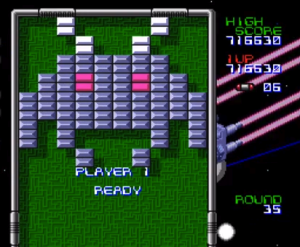
\includegraphics[width=0.7\textwidth]{images/estructura/niveles/ejemplo-arkanoid}
	\centering
	\caption{Homenaje a Space Invaders(Taito, 1978) dentro de Arkanoid: Doh it Again (Taito, 1997)}
	\label{ejemplo-arkanoid}
\end{figure}

En una primera versión, se planteó el uso del programa \textbf{Tiled}\footnote{http://www.mapeditor.org/}, un editor de mapas de propósito general que permite la edición de mapas basados en baldosas o \textbf{``tiles''} utilizando un sencillo procesador del lenguaje. Los mapas desarrollados generados con tiles eran exportados al formato \textbf{XML}, el cual podía se cargado en Unity. Sin embargo, al ser un programa de propósito general, Tiled contaba con mucha funcionalidad innecesaria que ralentizaba la producción de niveles, al mismo tiempo que carecía de ciertas funciones clave (como la selección individual de colores de bloques).

Finalmente, se optó por el sistema actual basado en imágenes dado que posibilita la producción rápida de niveles, fácilmente modificables con cualquier editor de imágenes. Adicionalmente, la implementación del sistema es capaz de ignorar pequeños errores en el mapa, como asignación de colores a casillas vacías o la presencia de colores que no se corresponden con ningún tipo de ladrillos, lo que reduce aún más los tiempos de producción.

Por otra parte, el sistema por imágenes tiene una serie de limitaciones que hay que tener en cuenta durante el diseño de niveles:
\begin{itemize}
  \item En primer lugar, \textbf{solo una pequeña cantidad de colores pueden ser asignados a tipos de ladrillos}. Esto se debe a las discrepancias entre los formatos de colores (los componentes RGB de los colores se guardan como enteros entre 0 y 255 en las texturas, pero como números de punto flotante entre 0 y 1 en la clase Color), la cual provoca perdida de información durante la conversión y nos fuerza a utilizar valores de color que sean fracciones exactas de 256. 
  \item En segundo lugar, el sistema no contempla la posibilidad de \textbf{rotar los ladrillos}. Debido a que esta funcionalidad era necesaria para la construcción de algunos niveles, fue necesario crear ladrillos prefabricados previamente rotados.
  \item En segundo lugar, se trata de un sistema poco escalable, permitiendo un tamaño único de campo de juego y poca capacidad para ``personalizar'' los tipos de bloque más allá de su color; por lo que sería necesario realizar cambios importantes en caso de que se necesitaran construir niveles más complejos
\end{itemize}

\subsection{Inicio del juego}
Cuando la escena de juego es cargada, el componente \textbf{Room} de la sala se encarga de coordinar la inicialización del juego. Este tiene asociadas referencias a la mayor parte de los objetos de la escena, lo que le permite llamar a los métodos correspondientes con facilidad. La secuencia de eventos del inicio del juego es la siguiente:

\begin{enumerate}
\item \textbf{Generación del nivel}: El componente Room invoca el método \textbf{Generate} del componente \textbf{LevelGenerator} iniciando la carga del nivel. Se trata de un proceso lento, por lo que puede tardar unos segundos. Sin embargo, la ralentización en la ejecución es camuflado con el efecto de cambio de escena.
\item \textbf{Entrada del jugador}: El \textbf{Personaje Principal} entra en la sala a través de la pared sur. El personaje principal inicia esta acción automáticamente al cargarse la sala y una vez alcanza el centro de la sala, se detiene y realiza invoca al método \textbf{PlayerReady} de Room para notificar que su entrada ha finalizado.
\item \textbf{Entrada del jefe}: Si se trata de un nivel de jefe, el jefe comienza su entrada en la sala. Al igual que el jugador, el jefe invoca al método \textbf{BossReady} de Room una vez su animación ha terminado.
\item \textbf{Activación de la pelota}: Una vez que el jugador (y el jefe) han finalizado su entrada, Room invoca el método \textbf{Activate} de la pelota, provocando que se vuelva visible y comience con su movimiento. 
\item \textbf{Control del jugador}: Inmediatamente después de activar la pelota, le componente Room invoca el método \textbf{Activate} del personaje principal, el cual empieza a reaccionar a las órdenes del jugador comienza el juego.
\end{enumerate}

\subsection{Condiciones de fin del juego}
Una vez finalizada la introducción, se da paso a la etapa de \textbf{Juego}. Esta etapa continua hasta que se alcanza un \textbf{estado de victoria o de derrota}, en los cuales el componente Room de la sala ejecuta una serie de eventos de fin del juego que culminan en un cambio de escenas.

El \textbf{estado de victoria} tiene lugar cuando la puerta de la sala se queda sin puntos de vida. Cuando esta condición se cumple, empieza la siguiente secuencia de acciones:
\begin{enumerate}
\item \textbf{Ocultar pelota}: Cuando la pelota golpea la puerta y esta no le quedan más puntos de vida, la pelota detiene su movimiento y desactiva tanto su collider como su renderer, provocando que se vuelva invisible e intangible.
\item \textbf{Animación de la puerta}: Al recibir un golpe y quedarse con cero puntos de vida, la puerta inicia su animación de apertura.
\item \textbf{Romper los ladrillos}: Cuando acaba la animación de la puerta, esta llama al método \textbf{DestroyBricks} del componente Room, lo que provoca que los ladrillos aun en pie sean destruidos.
\item \textbf{Salida del personaje principal}: Una vez finalizada la animación de la puerta, esta llama al método \textbf{WinCinematic} del personaje principal para que este salga de la sala por la puerta.
\item \textbf{Cambio de escena}: Cuando el personaje principal se ha alejado lo suficiente de la sala, este llama al método \textbf{NextStage} de la sala, lo que provoca un cambio de escena. Si se trataba del ultimo nivel, se carga la \textbf{escena de victoria}, si no, se vuelve a cargar la escena de juego, incrementando el índice de nivel.
\end{enumerate}

El \textbf{estado de derrota} se alcanza cuando la pelota golpea tres veces consecutivas el suelo de la sala. Cuando esta condición se cumple, empieza la siguiente secuencia de acciones:
\begin{enumerate}
\item \textbf{Destrucción de la Pelota}: La pelota comienza su animación de destrucción
\item \textbf{Derrota del jugador}: Cuando la pelota acaba su animación, se envía un mensaje al jugador para que comience con su animación de derrota.
\item \textbf{Cambio de escena}: Cuando termina la animación de la pelota, esta llama al método \textbf{GameOver} de la sala, el cual inicia la transición a la \textbf{escena de fin del juego}
\end{enumerate}

\section{Control del jugador}
El \textbf{personaje principal} es el avatar del jugador dentro del juego y puede controlarlo directamente pulsando teclas del teclado. El aspecto de este personaje es el de un pequeño robot (figura \ref{player_model}).
\begin{figure}[h]
	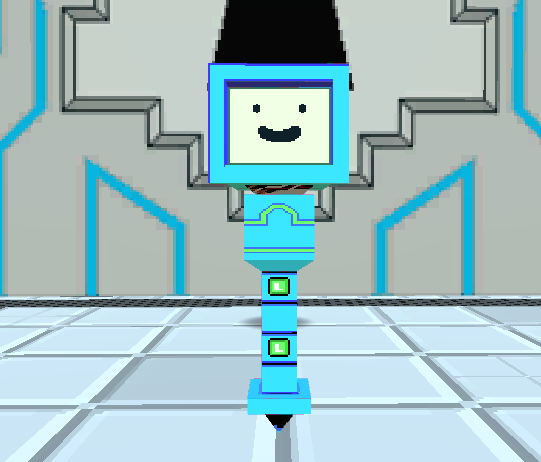
\includegraphics[width=0.85\textwidth]{images/estructura/personaje/flick_happy_small}
	\centering
	\caption{Modelo del personaje principal.}
	\label{player_model}
\end{figure}

El comportamiento del personaje principal es bastante sencillo: 
\begin{itemize}
\item Cuando el jugador pulsa las flechas de dirección, el personaje \textbf{se mueve hacia dicha dirección a velocidad constante}.
\item Cuando el jugador pulsa la tecla espacio, el personaje \textbf{despliega una ``paleta''} frente a él. El jugador debe utilizar esta paleta para redirigir la pelota. La paleta desaparece tras unos segundos, durante los cuales el personaje no puede moverse
\item Si la pelota golpea al personaje principal, este \textbf{se queda aturdido} unos segundos durante los cuales no obedecerá las instrucciones del jugador.
\end{itemize}
En adición a su comportamiento habitual, el personaje tiene tres \textbf{animaciones cinemáticas} que se utilizan al principio y final de los niveles del juego. Estas animaciones se reproducen cuando empieza un nivel, cuando el jugador supera un nivel y cuando el jugador pierde. Durante las animaciones, el jugador no puede controlar al personaje

\subsection{Componentes}
El personaje principal está implementado mediante dos GameObjects anidados (ver figura \ref{diagrama_personaje}). El \textbf{GameObject padre} contiene la lógica del personaje, determinada por los componentes que este tiene asociados.
\begin{itemize}
	\item Un \textbf{Rigidbody}. Este componente permite dotar al personaje de un comportamiento \textbf{basado en físicas}. El componente almacena las propiedades físicas del personaje (velocidad, aceleración, gravedad...) e implementa métodos para poder aplicarle fuerzas y cambios de velocidad.
	\item Un \textbf{Collider}. Este componente se utiliza en la \textbf{detección de colisiones} entre el personaje principal y el resto de los objetos de la escena. En concreto, el personaje principal tiene asociado un \textbf{BoxCollider}, el cual tiene forma de prisma rectangular.
	\item Un \textbf{Audio Source}, es el componente encargado de reproducir los sonidos del personaje.
	\item Un \textbf{Animator}, el cual reproduce las animaciones del personaje principal. Las animaciones (realizadas en el propio editor de Unity) estar guardadas como ``clips'' que el Animator carga dependiendo del estado interno del personaje.
	\item Un \textbf{Script} de la clase \textbf{MainCharacter}, el cual se ocupa de recibir la información de entrada del jugador y usarla para determinar qué acciones deben realizar los demás componentes.
\end{itemize}
\begin{figure}[h]
	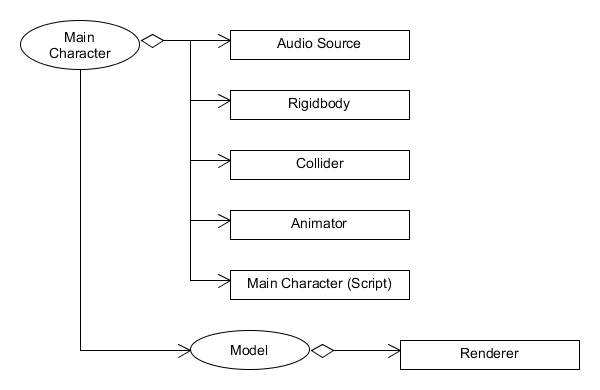
\includegraphics[width=0.8\textwidth]{images/estructura/personaje/main_character_objects}
	\centering
	\caption{Diagrama de componentes del personaje principal.}
	\label{diagrama_personaje}
\end{figure}

El \textbf{GameObject hijo} se encarga únicamente de contener renderizar el modelo del personaje a través del componente \textbf{MeshRenderer}. El motivo de esta división es un conflicto entre los componentes \textbf{Rigidbody y Animator} del GameObject principal debido a que ambos manipulan la rotación y posición del personaje, por lo que fue necesario mover el modelo a un objeto anidado. De esta forma, el rigidbody manipula la \textbf{posición y rotación globales} del personaje, mientras que el Animator controla las \textbf{propiedades locales} del objeto anidado.

Adicionalmente al objeto principal se encuentra la \textbf{Paleta} (figura \ref{paddle}). Se trata de un GameObject muy sencillo que cuenta con solo dos componentes: un \textbf{Renderer} y un \textbf{BoxCollider}. La paleta está guardada como \textbf{Prefab} en los assets del juego, de forma que el personaje principal puede instanciarla cuando sea necesario.
\begin{figure}[h]
	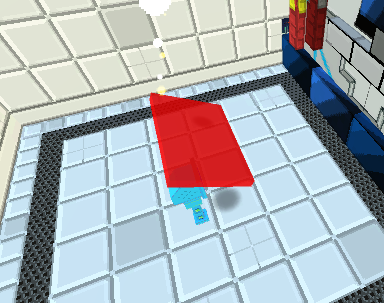
\includegraphics[width=0.8\textwidth]{images/estructura/personaje/flick_paddle}
	\centering
	\caption{Personaje principal activando la paleta}
	\label{paddle}
\end{figure}

\subsection{Comportamiento del personaje}
El componente \textbf{MainCharacter} es el encargado de coordinar el comportamiento del resto de componentes del personaje principal. Para ello, MainCharacter lee la entrada del jugador, procesa las teclas pulsadas y usa esa información para llamar a los métodos pertinentes del resto de componentes.  

El comportamiento de MainCharacter se basa en una \textbf{Maquina de Estados Finitos}, dado que las distintas acciones que el personaje puede realizar pueden modelarse muy bien como estados independientes, lo que además permite prevenir y aislar mejor los fallos de programación durante el desarrollo. En la figura \ref{player_states} se encuentran el diagrama de estados, los cuales se describen a continuación:
\begin{figure}[h]
	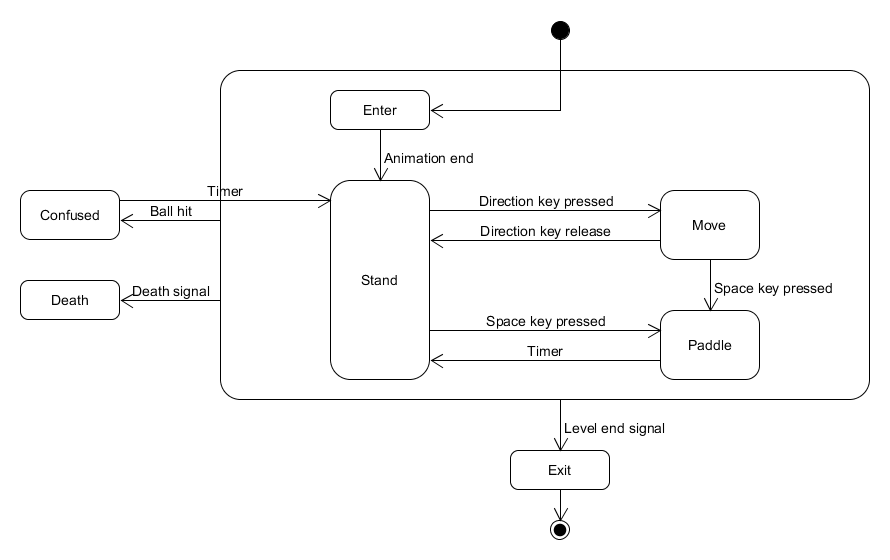
\includegraphics[width=0.95\textwidth]{images/estructura/personaje/main_character_states}
	\centering
	\caption{Diagrama de estados del personaje principal}
	\label{player_states}
\end{figure}

El estado \textbf{Enter} es el estado inicial del personaje. En este estado el personaje avanza desde el exterior de la sala hacia el centro de esta. Una vez alcanzado el centro de la sala, el personaje pasa al estado \textbf{Stand}. El desplazamiento se realiza mediante el componente \textbf{Rigidbody}, modificando el parámetro de la velocidad a un valor constante Durante este estado, el \textbf{Collider} se encuentra desactivado, para evitar que el jugador choque con las paredes de la sala.

El estado \textbf{Stand} es el estado por defecto del personaje, el que se encuentra activo cuando no se detecta ninguna pulsación de teclas ni interacciones con otros objetos. En este estado, el personaje permanece inmóvil ejecutando su animación de espera. El personaje cambiará de estado cuando detecte una pulsación de teclas: al estado \textbf{Move} si se han pulsado las flechas de dirección y al estado \textbf{Paddle} si se ha pulsado la tecla espacio.

En estado \textbf{Move} el personaje se mueve a velocidad constante en la dirección determinada por las flechas de dirección que el jugador esté pulsando. El componente se encarga de generar un vector que apunta a en la dirección resultante de sumar las direcciones de las flechas pulsadas, el cual se introduce como parámetro en el método \textbf{AddForce} del componente Rigidbody. El método AddForce aplica una fuerza determinada por el vector suministrado al objeto provocando su desplazamiento. Se utiliza este método en lugar de modificar la velocidad directamente porque así se obtiene una ligera aceleración inicial, que es mucho más agradable y natural para el jugador. La fuerza que utiliza para el movimiento es muy alta y va acompañada de un factor de fricción también elevado, lo que permitía controlar al personaje con precisión.

El estado \textbf{Paddle} el personaje instancia una \textbf{paleta} frente a él. Al mismo tiempo que se instancia la paleta comienza una cuenta atrás de unos segundos, tras los cuales la paleta se destruye y el personaje retorna al estado \textbf{Stand}. Durante la ejecución de este estado, el jugador no podrá controlar el movimiento del jugador, sin embargo, la fricción entre el personaje y el suelo de la sala se reduce en este estado, por lo que el personaje conservará parte de la velocidad que tuviese en estados anteriores gracias a la inercia.

El personaje entra en el estado \textbf{Confused} cuando es golpeado por la pelota, independientemente de en qué estado se encontrase antes. El personaje permanecerá en este estado durante unos segundos mientras el \textbf{animator} ejecuta una animación de mareo. Finalizado el estado, el jugador volverá al estado \textbf{Stand}.

El estado \textbf{Dead} comienza cuando el personaje recibe una llamada a su método \textbf{Dead}, es cual sirve para notificarle de la destrucción de la pelota. Este método esta siempre activo, por lo que el personaje puede entrar en este estado desde cualquier otro. Al entrar en este estado, el \textbf{Animator} reproduce la animación de muerte del personaje, en la que este se desploma derrotado y se queda inmóvil. La lectura de entrada queda desactivada, por lo que el jugador pierde el control sobre el personaje.

El estado \textbf{Exit} empieza cuando se llama al método \textbf{WinCinematic} del personaje. Esta llamada se produce cuando el jugador supera el nivel actual. Durante este estado, el personaje avanza hacia el frente, atravesando la puerta de la sala (ahora abierta) y creando la ilusión de que ``avanza al siguiente nivel´´. Este movimiento del jugador se implementa de la misma forma que el del estado \textbf{Move}, usando el método \textbf{AddForce} del componente RigidBody.

\section{Físicas e interacción}
La dinámica de este juego surge principalmente de las \textbf{interacciones físicas entre los distintos objetos} contenidos en la sala. Obviando las simples colisiones entre el personaje y la sala que sirven para evitar que este no abandone la sala, todas las colisiones se producen entre \textbf{la pelota} y otro objeto. Cada objeto de la sala reacciona de forma distinta al impacto con la pelota.

En los siguientes apartados se describirá en detalle a la pelota, así como los distintos objetos que pueden colisionar con esta.

\subsection{Pelota}
Podríamos considerar \textbf{la pelota} como \textbf{el arma del personaje principal}, el medio por el que el jugador interacciona con los objetos del juego. La pelota viaja en trayectoria rectilínea, rebotando en las paredes y el techo de la sala del juego. Al golpear la puerta, o los bloques que la cubren, estos reciben daño y la pelota rebota, pero si la pelota golpea el suelo de la sala es ella la que recibe daño, no el jugador. Si la pelota golpea el suelo tres veces, esta se destruye y partida se acaba. El jugador debe intentar golpear la pelota con la paleta para redirigiría hacia la puerta, evitando que toque el suelo.

Visualmente, la pelota es una simple esfera de color uniforme, como puede verse en la figura \ref{ball}. Para facilitarle al jugador la tarea de seguir la trayectoria de la pelota, esta va dejando a su paso un rastro luminoso y produce con cada colisión un efecto visual de impacto.
\begin{figure}[h]
	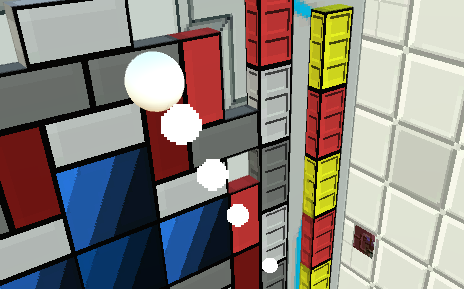
\includegraphics[width=0.65\textwidth]{images/estructura/fisica/ball_moving}
	\centering
	\caption{Pelota moviéndose}
	\label{ball}
\end{figure}

\subsubsection{Componentes}
La pelota está implementada mediante dos \textbf{GameObject} anidados. El primer GameObject tiene asociados una serie de componentes que modelan su comportamiento (la estructura de componentes puede verse en la figura \ref{ball_object}. Estos componentes son:
\begin{itemize}
\item Un \textbf{MeshRenderer} encargado de renderizar el modelo de la bola, el cual es una sencilla esfera con una textura lisa.
\item Un \textbf{SphereCollider} que se utiliza para la detección de colisiones entre la pelota y el resto de los objetos de la sala.
\item Un \textbf{Rigidbody} que sirve para dotar a la pelota de propiedades físicas.
\item Un \textbf{Audio Source}, el cual reproduce los sonidos de impacto entre la pelota y los otros objetos.
\item Un \textbf{Animator} para ejecutar la animación de destrucción de la bola.
\item Un \textbf{Particle System}, un componente que permite crear animaciones y efectos especiales utilizando \textbf{partículas}, pequeños gráficos bidimensionales. En la pelota, el ParticleSystem se utiliza para crear una \textbf{trayectoria} que marca el camino que siguió la pelota.
\item Un \textbf{Script} de la clase \textbf{Ball} que controla el comportamiento de la bola, determinando su estado y determinando que reacción debe ejecutar cuando colisiona con otros objetos.
\end{itemize}

\begin{figure}[h]
	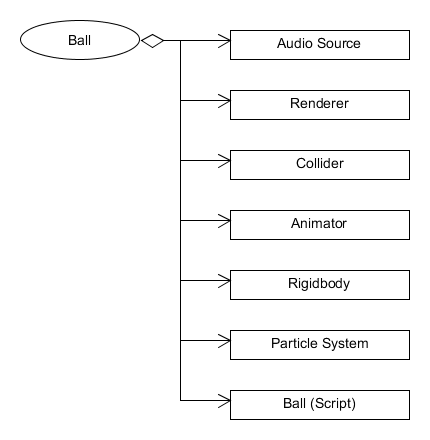
\includegraphics[width=0.65\textwidth]{images/estructura/fisica/ball}
	\centering
	\caption{Componentes del objeto Ball.}
	\label{ball_object}
\end{figure}

Anidado a este primer GameObject se encuentra el \textbf{emisor de sombra}. La función de este GameObject es la de producir una sombra esférica contra el suelo de la sala gracias a su componente \textbf{Proyector}. El motivo por el que se emplea este componente en lugar de utilizar es sistema de iluminación de Unity para crear la sombra es que no se busca crear una sombra realista de la pelota, sino una referencia en el suelo de la posición de la pelota que permita al jugador seguirla más fácilmente. Si se quisiese obtener el mismo efecto con el sistema de iluminación sería necesario utilizar una configuración de luces muy especifica que desmejoraría el reto de gráficos.

Adicionalmente, la pelota tiene acceso a dos objetos prefabricados que implementan sus efectos visuales: \textbf{ParticleCircle} y \textbf{ExplosionParticle}. ParticleCircle genera una explosión de partículas en forma de anillo mientras que ExplosionParticle genera una explosión esférica. Ambos objetos tienen un solo componente: un ParticleEmitter ya que es la pelota la encargada de completar el resto de sus funciones. En la figura \ref{particles} pueden verse los efectos de ambos objetos.
\begin{figure}[!htb]
   \begin{minipage}{0.48\textwidth}
     \centering
     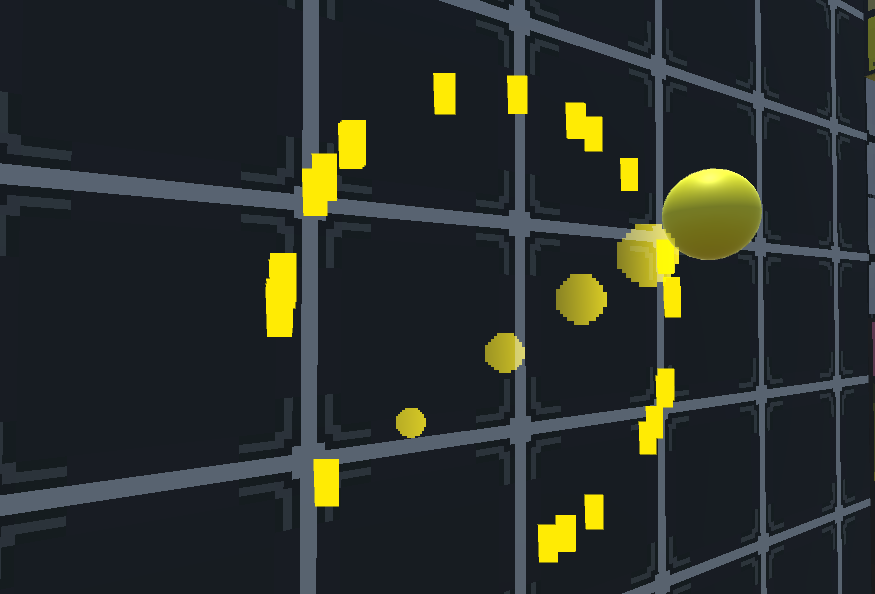
\includegraphics[width=0.8\linewidth, right]{images/estructura/fisica/ball_hit}
   \end{minipage}\hfill
   \begin {minipage}{0.48\textwidth}
     \centering
     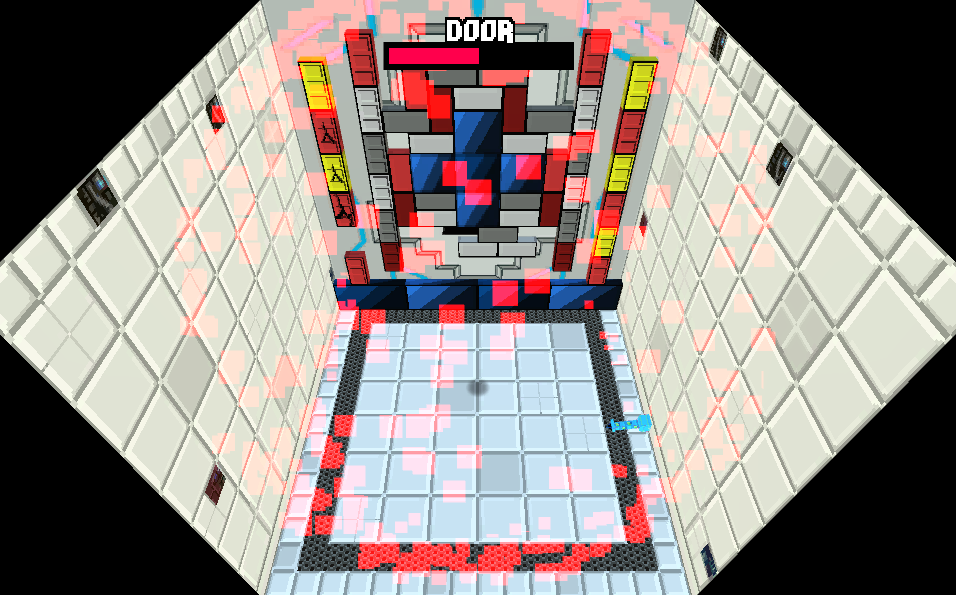
\includegraphics[width=0.8\linewidth, left]{images/estructura/fisica/ball_explosion}
   \end{minipage}
   \caption{ParticleCircle (izquierda) y ExplosionParticle (derecha)}
   \label{particles}
\end{figure}

\subsubsection{Comportamiento}
El componente \textbf{Ball} es el encargado de dotar a la pelota de su comportamiento. Su funcionamiento se basa en una máquina de estados finitos con un total de tres estados: \textbf{Normal}, \textbf{Locked} y \textbf{Destroy}.

Los estados \textbf{Locked} y \textbf{Destroy} son estados cinemáticos utilizados durante las secuencias de inicio y final del nivel. Durante el estado \textbf{Locked} la pelota tiene desactivados sus componentes \textbf{Renderer}, \textbf{Rigidbody} y \textbf{Collider}, por lo que es inmóvil, invisible e intangible. Este es el estado en el que la pelota se encuentra durante las secuencias de introducción y de victoria. Por otro lado, durante el estado \textbf{Locked} el componente \textbf{Animator} de la pelota reproduce una animación de destrucción, que culmina con la instanciación de un \textbf{ExplosionParticle}. Este es el estado que utiliza la pelota durante la derrota.

Durante el resto de la ejecución, la pelota se encuentra en el estado \textbf{Normal}. En este estado, la pelota se mueve a velocidad constante por la sala rebotando en los diversos objetos contenidos en esta, así como en sus paredes, suelo y techo. El movimiento de la pelota se consigue gracias al componente \textbf{Rigidbody}. Al entrar en el estado \textbf{Normal}, la pelota recibe un impulso en una dirección aleatoria mediante el método \textbf{AddForce} del rigidbody y a partir de ahí se moverá de forma perpetua al haber sido configurada sin fricción.

Cuando la pelota colisiona con otro objeto físico, esta debe determinar de qué tipo de objeto se trata para poder producir la reacción correspondiente. La identificación de los objetos se consigue gracias a sus \textbf{Tags}, un atributo presente en todos los GameObjects que permite distinguirlos rápidamente. Una vez que la pelota a determinado de qué tipo de objeto se trata, un método con las acciones convenientes.

La pelota tiene también un \textbf{contador de golpes}. Cuando este contador llega a tres, la pelota es destruida y el jugador pierde la partida. El contador de golpes también sirve para determinar el \textbf{color} de la pelota: blanca si no ha recibido golpes, amarilla si ha recibido uno y roja si ha recibido dos o más. 

\subsection{Elementos Interactivos}
\subsubsection{Paredes y Suelo}
Las paredes, el suelo y el techo son objetos hijos de la sala. Estos objetos carecen de comportamiento en sí mismo, pero pueden producir cambios en el comportamiento de la pelota cuando esta choca con ellos.

Si la pelota choca contra \textbf{las paredes} de la sala, cambiará de dirección rebotando de forma natural. Al no tener fricción, la pelota conservará su velocidad tras el rebote. Este comportamiento no se encuentra codificado dentro del componente \textbf{Ball}, sino que se trata de la consecuencia de las propiedades físicas del componente \textbf{Rigidbody}. A efectos prácticos, el techo de la sala es otra pared más, con un comportamiento idéntico al de las otras paredes.

Sin embargo, el comportamiento de la pelota cuando golpea el \textbf{suelo} de la sala es distinto. Al impactar contra el suelo, el contador de golpes se incrementará en uno. Para paliar el efecto negativo de este tipo de colisión, tras el impacto la pelota en \textbf{dirección a la puerta} de la sala. De esta forma, aunque el jugador haya se encuentre más cerca de perder la partida, tendrá más posibilidades de reponerse dado que se le ha ``regalado'' un golpe adicional  a la puerta. 

\subsubsection{Personaje Principal}
El objetivo principal del jugador es conseguir que el personaje principal \textbf{golpee la pelota con la paleta}. La dirección hacia la que rebote la pelota tras la colisión depende del punto de la paleta en el que se produjo el impacto, en lugar de en el ángulo de colisión. La trayectoria de salida de la pelota será más perpendicular al plano de la paleta cuanto más cerca de su centro se encuentre, y más paralela cuanto más alejado del centro sea. En la figura \ref{paddle_direction} se pueden ver de forma aproximada las trayectorias.
\begin{figure}[!htb]
   \begin{minipage}{0.5\textwidth}
     \centering
     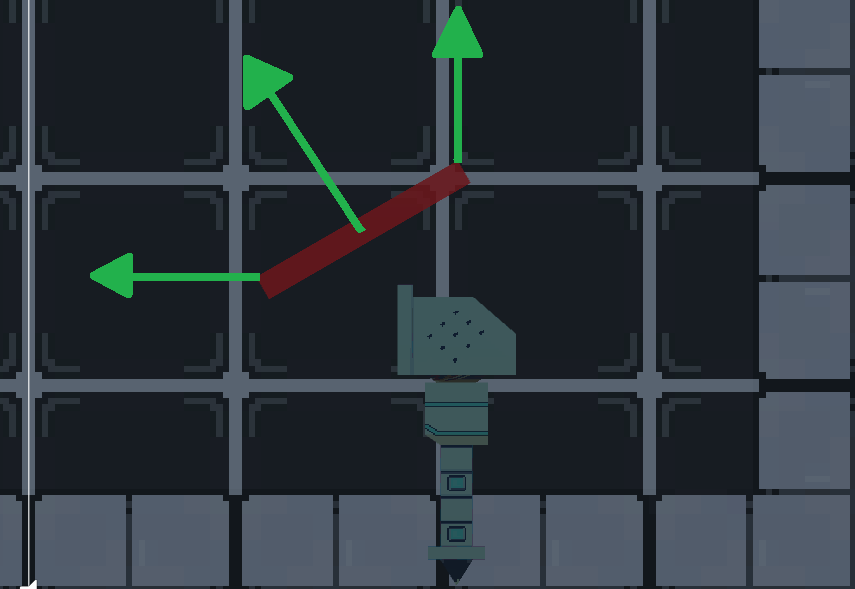
\includegraphics[width=0.9\linewidth, right]{images/estructura/fisica/paddle_direction_side}
   \end{minipage}\hfill
   \begin {minipage}{0.5\textwidth}
     \centering
     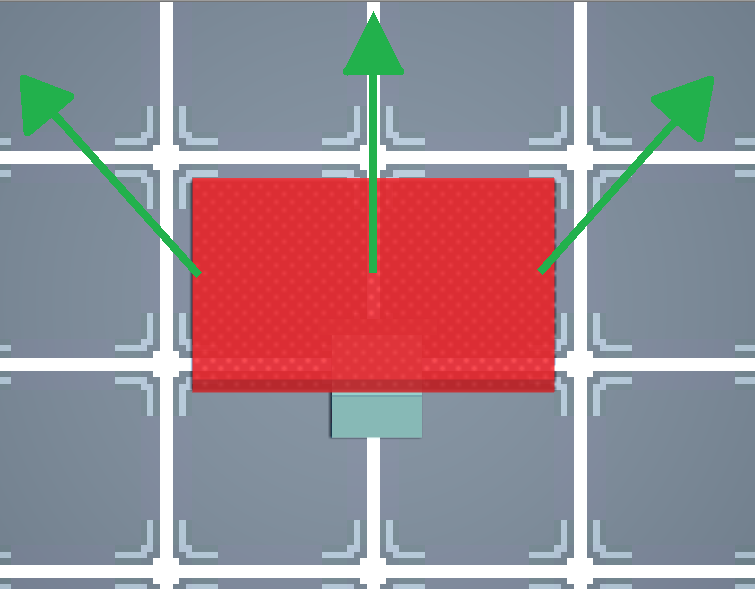
\includegraphics[width=0.9\linewidth, left]{images/estructura/fisica/paddle_direction_top}
   \end{minipage}
   \caption{Direcciones que tomaría la pelota dependiendo del punto de la paleta que golpee (Aproximada)}
   \label{paddle_direction}
\end{figure}

Por otro lado, si la pelota golpea al \textbf{personaje principal} directamente, este se quedará aturdido unos instantes. Tras el impacto, la pelota rebotará de forma natural.

\subsubsection{Puerta}
La \textbf{puerta} es una estructura que ocupa la pared norte de la sala (figura \ref{puerta}). El objetivo del juego es el de abrir la puerta golpeándola con la pelota. La puerta tiene un contador de \textbf{puntos de vida} que disminuye con cada impacto de la pelota. Cuando el contador llega a cero, la puerta se abre y el nivel se acaba. Además de con el descenso de sus puntos de vida, la puerta reaccionara a los impactos de la pelota moviendo sus paneles.
\begin{figure}[h]
	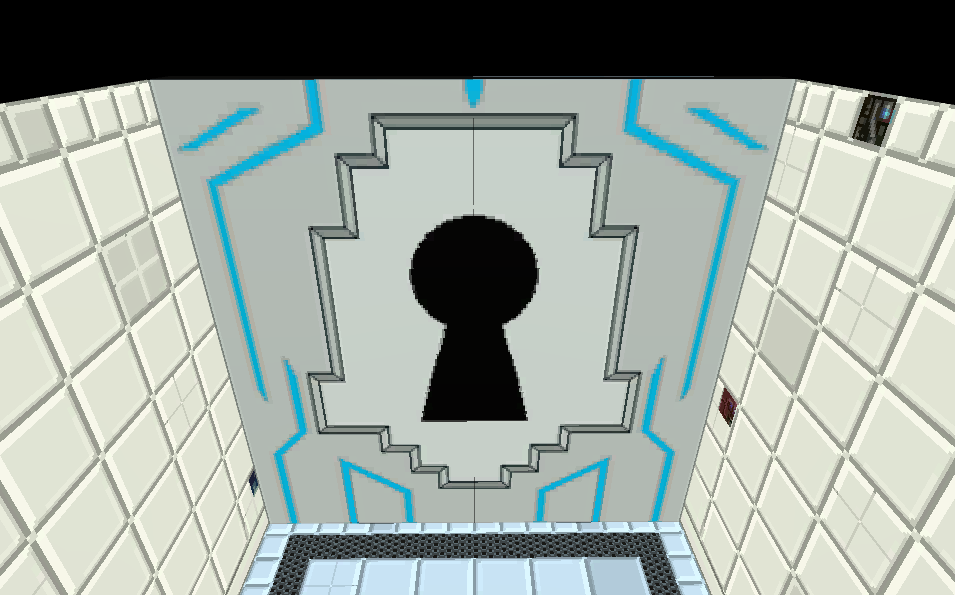
\includegraphics[width=0.8\textwidth]{images/estructura/fisica/puerta}
	\centering
	\caption{Modelo de la puerta.}
	\label{puerta}
\end{figure}

El GameObject que se utiliza para implementar la puerta se encuentra \textbf{anidado dentro de la sala}. La puerta tiene a su vez dos objetos anidados que hacen de paneles de la puerta. Los componentes de la puerta son:
\begin{itemize}
\item Un \textbf{BoxCollider} utilizado en la detección de colisiones.
\item Un \textbf{Animator} que se encarga de reproducir las animaciones de la puerta
\item Un \textbf{Script} de la clase \textbf{Door} la cual se encarga de gestionar el comportamiento de la puerta.
\end{itemize}
EN la figura \ref{puerta_diagrama} se puede ver de forma gráfica esta relación de objetos.
\begin{figure}[h]
	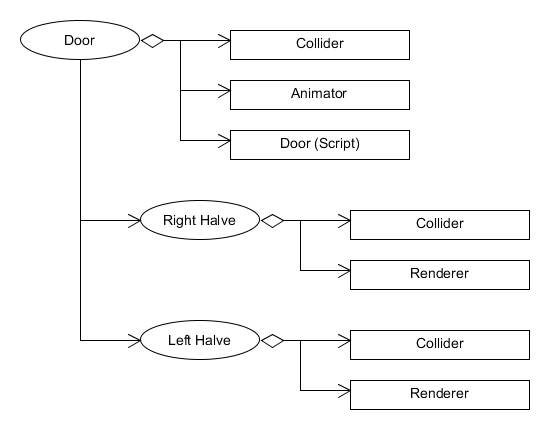
\includegraphics[width=0.8\textwidth]{images/estructura/fisica/door}
	\centering
	\caption{Diagrama de componentes de la puerta.}
	\label{puerta_diagrama}
\end{figure}

Cuando la pelota impacta con la puerta, esta llama al método \textbf{DoDamage} del componente \textbf{Door} de la puerta. Este método disminuye los puntos de vida de la puerta, inicia la animación de golpe y, en caso de que la puerta tenga cero puntos de vida, inicia la animación de apertura de la puerta.

Tras impactar con la puerta, la pelota rebotara de forma natural. Adicionalmente, el parámetro \textbf{UseGravity} del Rigidbody de la pelota cambiará su valor a verdadero, por lo que la pelota empezará a caer en dirección al suelo de la sala. La gravedad de la pelota no se desactivará hasta que no golpee el suelo de la sala o la paleta del jugador.

\subsubsection{Ladrillos}
Los \textbf{ladrillos} son el principal obstáculo del juego, ya que protegen la puerta de los golpes de la bola. Cada vez que la pelota golpea un ladrillo, este pierde un punto de vida. Cada ladrillo tiene asignado un \textbf{color} que tiñe su textura. Cuando sus puntos de vida llegan a cero, el ladrillo se destruye. Los ladrillos se colocan delante de la puerta, en una \textbf{cuadricula} de 16 X 16 casillas. Cada nivel del juego tiene una configuración de ladrillos diferente. 

Para darle variedad al juego, existen varios tipos de ladrillos (ver figura \ref{bricks_models}:
\begin{itemize}
\item \textbf{Ladrillo básico}: Es el ladrillo básico. Solo tiene un punto de vida. Este ladrillo mide 1 X 2 casillas.
\item \textbf{Ladrillo Multi-golpe}: Este ladrillo tiene tres puntos de vida, por lo que es más difícil romperlo. La textura de este ladrillo cambia con cada golpe para mostrar el daño infligido. Este ladrillo mide 1 X 2 casillas.
\item \textbf{Ladrillo Divisible}: Es un ladrillo de gran tamaño, mide 2 X 2 casillas. Aunque solo tiene un punto de vida, al romperse genera 4 ladrillos pequeños de 1 X 1 casillas de tamaño.
\item \textbf{Ladrillo Pequeño}: es un ladrillo idéntico al básico, salvo porque solo mide 1 X 1 casillas. Solo aparecen como resultado de la rotura de un ladrillo divisible.
\item \textbf{Ladrillo Irrompible}: Como su nombre indica, este ladrillo no puede ser destruido por la pelota. Miden 2 X 3 Casillas.
\end{itemize}
\begin{figure}[h]
	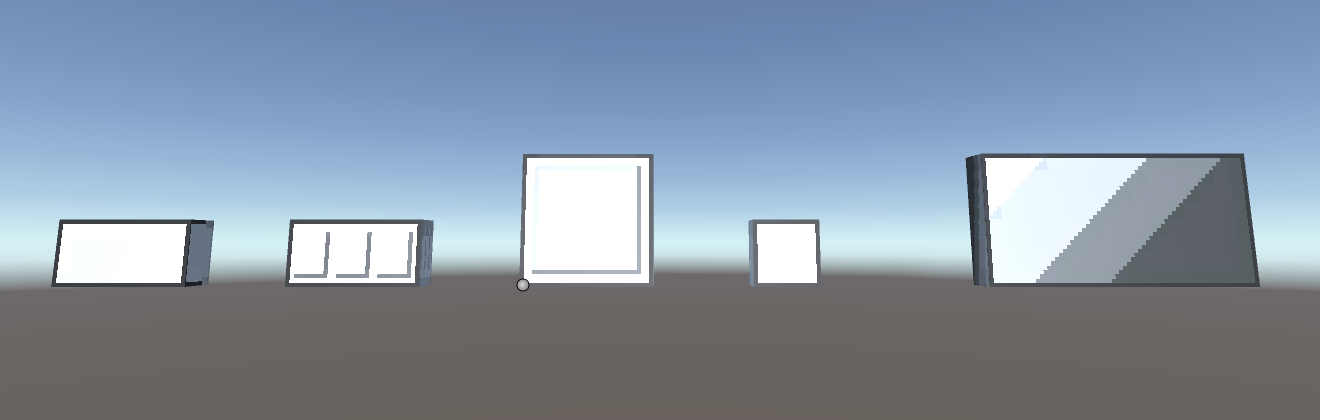
\includegraphics[width=0.65\textwidth]{images/estructura/fisica/brick_examples}
	\centering
	\caption{Modelos de los ladrillos}
	\label{bricks_models}
\end{figure}

Para implementar los ladrillos se utilizan dos GameObjects anidados, como se muestra en \ref{diagrama_brick}. El primer GameObject se encarga de dotar al ladrillo de funcionalidad, mientras que el segundo contiene el modelo 3D del mismo. Los componentes que contienen los ladrillos son los siguientes: 
\begin{itemize}
\item Un \textbf{BoxCollider}, para la detección de colisiones.
\item Un \textbf{Particle System}, para la animación de destrucción.
\item Un \ un script de clase \textbf{Brick}, que contiene la funcionalidad del ladrillo.
\end{itemize}
\begin{figure}[h]
	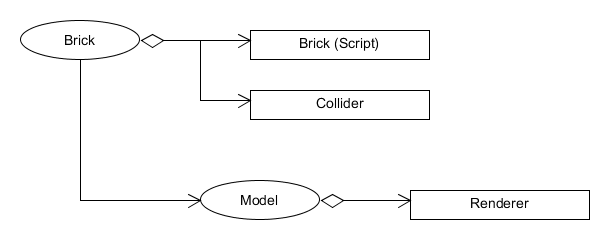
\includegraphics[width=0.65\textwidth]{images/estructura/fisica/bricks}
	\centering
	\caption{Componentes del objeto Brick.}
	\label{diagrama_brick}
\end{figure}

Cuando la pelota impacta contra un ladrillo, llama al método \textbf{DoDamamge} de su componente \textbf{Brick}. Este método recibe como parámetro una cantidad de ``puntos de daño'' la cual sustrae a los puntos de vida actuales del ladrillo. Además, este método también destruye los ladrillos que han perdido todos sus puntos de vida y emite partículas del color del ladrillo con cada golpe recibido. 

Los ladrillos básicos tendrían el comportamiento anteriormente distinto, pero el resto de los tipos de ladrillos requieren comportamientos específicos. De la clase \textbf{Brick} heredan tres clases hijas con código adicional para poder implementar todos los tipos de ladrillos, tal y como aparece en la figura \ref{brick_classes}. Estas clases son:
\begin{itemize}
\item \textbf{TextureChangeBrick}: Este script cambia la textura del ladrillo dependiendo del número de puntos de vida. Se utiliza en los \textbf{ladrillos multi golpes} para mostrar el ladrillo en varios estados de destrucción.
\item \textbf{DivisibleBrick}: Este componente se utiliza en la implementación de los \textbf{ladrillos divisibles}. Cuando este tipo de ladrillos se destruye, el componente instancia cuatro \textbf{bloques pequeños}.
\item \textbf{UnbreakableBrick}: Este componente ignora las llamadas de la bola, por lo que el ladrillo no pierde puntos de vida. Se utiliza en los \textbf{ladrillos irrompibles}
\end{itemize}
\begin{figure}[h]
	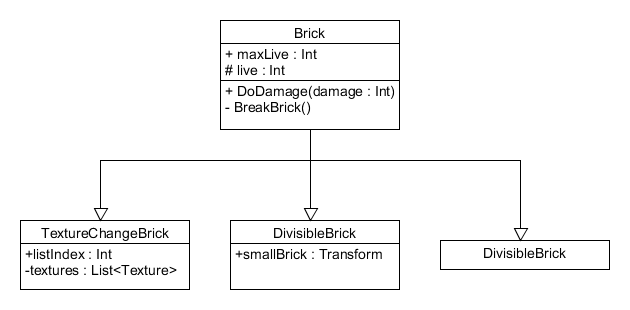
\includegraphics[width=0.65\textwidth]{images/estructura/fisica/brick_classes}
	\centering
	\caption{Jerarquía de clases de Brick.}
	\label{brick_classes}
\end{figure}

La reacción de la pelota al golpear un ladrillo es idéntica a la que tiene cuando golpea la puerta: la pelota rebotará de forma natural, pero se activará su \textbf{gravedad}, por lo que la pelota empezará a caer en dirección al suelo de la sala. De la misma manera, la gravedad de la pelota permanecerá activa hasta que golpee el suelo o la paleta.

\section{Jefe Final}
Un \textbf{jefe final}, o monstruo jefe, es un enemigo poderoso al que los jugadores deben enfrentarse para poder alcanzar algún objetivo dentro del juego \cite{game_design_patterns}. Los jefes sirven principalmente para tres propósitos: dar clausura a una sección del juego, al colocarse al final de una sección, nivel o fase; ofrecen variedad al juego, al cambiar las mecánicas de juego; y finalmente sirven como ``test'' para el jugador, al tratarse de un desafió mucho mayor que los anteriores. 

Para este juego, el jefe final es el único ``enemigo'' al que se enfrenta el jugador, que aparece en el nivel 11 del juego. Este jefe se comporta como un \textbf{``clon''} o ``rival'' del jugador: su objetivo es impedir que la pelota golpee la puerta, moviéndose y redirigiéndola de forma similar a como lo haría el jugador. La forma de derrotar a este jefe es idéntica de a como se supera cualquier fase: Golpeando la puerta suficientes veces. 

El jefe se mueve a \textbf{velocidad constante}, siempre pegado a la pared, intentando bloquear la pelota. Sin embargo, si detuviese siempre la pelota, sería un desafío imposible de superar, lo que no sería divertido para el jugador. La idea es que este jefe se juegue como si de una partida de tenis se tratase, con dos adversarios intercambiándose la pelota hasta que uno de los dos falle. Por ello, el jefe tendrá un \textbf{sistema de energía} que determinará su eficiencia a la hora de jugar e ira consumiéndose según avance la partida. En la figura \ref{boss} puede verse el modelo 3D de este enemigo.
\begin{figure}[h]
	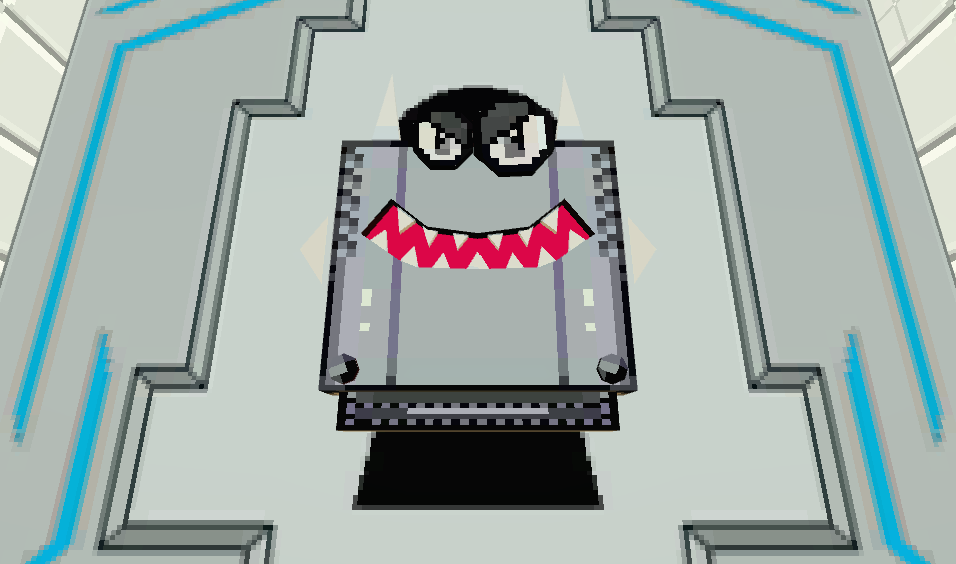
\includegraphics[width=0.70\textwidth]{images/estructura/jefe/boss-captura}
	\centering
	\caption{Modelo del jefe.}
	\label{boss}
\end{figure}

\subsection{Componentes}
Para implementar al jefe se utilizan \textbf{dos GameObjects anidados}. El GameObject principal contiene los componentes necesarios para el funcionamiento del jefe. Los componentes de este primer GamObject son los siguientes:
 \begin{itemize}
	\item Un \textbf{RigidBody} que sirve para dotar al jefe de \textbf{propiedades físicas}, como velocidad o aceleración.
	\item Un \textbf{BoxCollider} el cual permite realizar la detección de colisiones entre el jefe y otros objetos.
	\item Un \textbf{Animator} el cual dota al jefe de animaciones de modo que su comportamiento no resulte demasiado estático. 
	\item Un \textbf{Audio Source} que sirve para emitir sonidos y música. El jefe lo utiliza para emitir sonidos en situaciones concretas, como al golpear la pelota o al ser derrotado.
	\item Un \textbf{Script} de clase \textbf{BossController.} Este componente determina que movimientos es capaz de realizar el jefe.
	\item Un \textbf{Script} de clase \textbf{BossAI.} Este componente se encarga de controlar el comportamiento del jefe.
En la figura \ref{diagrama_boss} se pude ver un diagrama de este objeto y sus componentes.
\end{itemize}
\begin{figure}[h]
	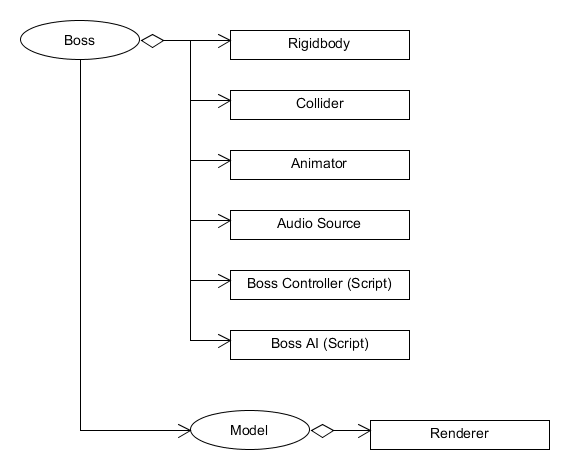
\includegraphics[width=0.8\textwidth]{images/estructura/jefe/boss}
	\centering
	\caption{Diagrama de componentes del jefe.}
	\label{diagrama_boss}
\end{figure}

El segundo GameObject contiene el modelo 3D del jefe, el cual es dibujado en pantalla gracias a un componente \textbf{MeshRenderer}. Esta separación se realizó para evitar colisión entre los comportamientos de los componentes \textbf{Rigidbody} y \textbf{Animator}.

El jefe no \textbf{forma parte de la escena del juego} al comienzo de la ejecución, sino que está almacenado en los assets del juego en forma de \textbf{Prefab}. El prefab es instanciado por el componente \textbf{LevelGenerator} de la sala durante la generación del nivel en el caso de que la información del nivel indique que se trata de un nivel del jefe. Al ser instanciado, el jefe es asignado como GameObject hijo de la puerta, de forma que su posición sea siempre relativa a esta.

El comportamiento del jefe se encuentra dividido en dos scripts para separar las acciones que puede realizar el jefe, implementadas en \textbf{BossController}) de la inteligencia artificial que determina cuales de esas acciones debe realizar en un momento dado (implementada en \textbf{BossAI}). 

\subsection{Movimiento}
El componente \textbf{BossController} contiene la información y las funciones que el jefe necesita para realizar sus acciones. Las acciones que el jefe puede realizar son \textbf{moverse}, modificar sus \textbf{valores de energía}, ser \textbf{activado y destruido} y \textbf{reproducir sonidos}.

El movimiento del jefe se produce mediante el método \textbf{MoveDirection}. Este método mueve al jefe a velocidad constante en la dirección suministrada como parámetro. La dirección del movimiento viene dada como un ángulo, el cual se utiliza para calcular el vector de dirección paralelo al plano de la puerta. El movimiento se implementa mediante el método \textbf{AddForce} del componente \textbf{Rigidbody} del jefe, de esta forma el movimiento tiene una aceleración inicial que lo hace más natural y además tiene en cuenta las colisiones con las paredes de la sala de forma automática.

La velocidad del movimiento del jefe está determinada por un \textbf{Sistema de energía}. La cantidad de energía se encuentra almacenada en la variable \textbf{energy}, la cual empieza inicializada con el mismo valor que el atributo \textbf{maxEnergy} de la clase. Para calcular la velocidad, se multiplica un valor de velocidad inicial por la proporción entre energy y una tercera variable llamada \textbf{baseEnergy} que contiene el valor inicial de maxEnergy. Para modificar las variables del sistema de energía se deben utilizar los métodos \textbf{DecrementEnergy}, que decrementa energy en el porcentaje introducido por parámetro, y \textbf{IncrementMaxEnergy}, que incrementa maxEnergy en el porcentaje introducido e iguala el valor de energy al nuevo valor de maxEnergy. Ambos métodos calculan también el nuevo valor de la velocidad .

El jefe incluye dos métodos que sirven para activar y detener su ejecución: \textbf{Activate} y \textbf{StartDestruction}. Ambos métodos funcionan modificando el valor de unas variables (active y destroy) que indican si el jefe se encuentra activo o si ha sido destruido. Estas variables son tomadas por el componente \textbf{animator} para determinar que animaciones reproducir.

Adicionalmente a su comportamiento más físico, el jefe tiene una serie de efectos de sonido que debe reproducir en momentos concretos de su comportamiento. Estos sonidos se reproducen mediante una serie de funciones públicas:
\begin{itemize}
\item PlayStartSound, que reproduce un ``rugido'' cuando el jefe entra en escena.
\item PlayBallSound, para el sonido de impacto entre la pelota y el jefe.
\item PlayHurtSound, que es el sonido que emite el jefe cuando la pelota golpea la puerta.
\item PlayDefeatSound, para el sonido que el emite al ser destruido.
\end{itemize}

\subsection{Inteligencia Artificial}
El componente \textbf{BossAI} implementa el patrón de comportamiento del jefe, determinando cuándo y en qué dirección debe moverse el jefe, que animación debe reproducirse y cuando reproducir los efectos de sonido. La separación de esta inteligencia artificial de la implementación de las acciones del jefe se realizó principalmente para facilitar su desarrollo: de esta forma se podía determinar en caso de error o de comportamientos no intencionados si se trataba de un problema de la inteligencia artificial o de la implementación del movimiento. Adicionalmente, este sistema en dos piezas permitiría cambiar la inteligencia artificial con facilidad para poder construir jefes con distintos comportamientos.

La función principal de la inteligencia artificial es la de mover al jefe en dirección a la pelota, de forma que pueda detenerla antes de que colisione con la puerta. Este movimiento se realiza a través del método \textbf{MoveDirection} el componente \textbf{BossController}, el cual requiere del ángulo del movimiento. La inteligencia artificial obtiene el ángulo con el método privado \textbf{AngleToBall}, el cual, usando la posición de la bola, el jefe, y el vector normal al plano de la puerta es capaz de calcular el ángulo entre el jefe y la proyección de la pelota en la superficie de la puerta.

El movimiento del jefe no es la única función de su inteligencia artificial. Para dar la impresión de que el jefe se comporta con una mínima inteligencia, su comportamiento incluye fases de reposo intercaladas entre las de movimiento, así como animaciones para su introducción en el nivel, para cuando recibe daño y para su destrucción. La implementación de estos comportamientos se realiza mediante una \textbf{máquina de estados finitos} (figura \ref{boss_states} dotada de los siguientes estados:
 \begin{itemize}
	\item \textbf{Out}: El jefe espera fuera del área de juego, inmóvil, a la espera de que la variable \textbf{Active} de \textbf{BossController} esté en ``verdadero''. 
	\item \textbf{Intro}: El jefe entra en la sala, moviéndose hacia su posición inicial en el centro de la sala. Acto seguido, el jefe realiza su animación inicial, moviéndose ligeramente y emitiendo sonidos. Este movimiento se implementa mediante el componente \textbf{Animator} en lugar de BossController ya que el jefe debe atravesar el techo solido de la sala.
	\item \textbf{Wait}: En este estado, el jefe permanece inmóvil a la espera de un estímulo que le haga cambiar al estado \textbf{Move}. El estímulo es que la pelota se mueva en dirección a la puerta. El jefe cuenta con un \textbf{tiempo de reacción}, por lo que una vez que entra en este estado deberá permanecer en el durante al menos ese tiempo antes de poder cambiar al estado \textbf{Move}
	\item \textbf{Move}: El jefe se mueve en dirección a la pelota utilizando los métodos de BossController. El movimiento se detendrá si se consigue golpear la pelota o si la pelota golpea la puerta. 
	\item \textbf{Hurt}: En este estado el jefe permanece inmóvil mientras se reproduce una animación de daño. Tras esta breve pausa, el jefe retorna al estado \textbf{Wait}.
	\item \textbf{Death}: Cuando la puerta se abre, el jefe realiza una animación de destrucción mediante el componente \textbf{Animator}, para después volverse invisible mientras produce una explosión de partículas (instanciando un objeto de la clase \textbf{ParticleExplosion}. 
\end{itemize}
\begin{figure}[h]
	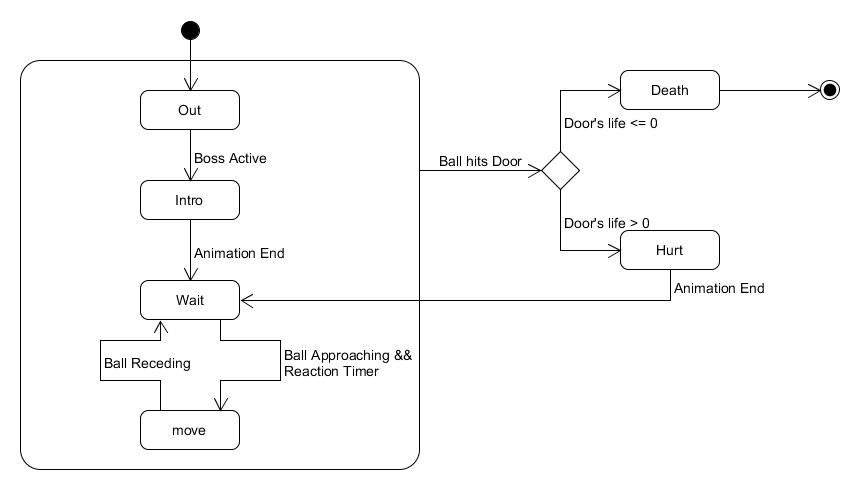
\includegraphics[width=1\textwidth]{images/estructura/jefe/boss-estados}
	\centering
	\caption{Diagrama de estados del jefe.}
	\label{boss_states}
\end{figure}

\section{Patrones de Diseño}
Un \textbf{Patrón de diseño} es, en el contexto de la ingeniería de software, una solución reutilizable para un problema frecuente. Los patrones de diseño se presentan como descripciones o plantillas de cómo debe resolverse el problema más que como fragmentos de código que puedan añadirse directamente a un programa, de modo que el programador pueda aplicarlos a distintos contextos dependiendo de sus necesidades.

El concepto de patrón de diseño aplicado al diseño de software surgió en el libro \textbf{Design Patterns: Elements of Reusable Object-Oriented Software} \cite{design_patterns}, donde se introduce no solo la idea de los patrones de diseño, sino también algunos de los patrones más utilizados como \textbf{Singleton} o \textbf{Abstract Factory}. Este libro se inspira en una obra anterior llamada \textbf{A Pattern Language} de Christopher Alexander, una obra de estructura similar en la que se describen patrones de diseño en arquitectura \cite{game_programming_patterns}.

En los siguientes apartados se describirán los patrones de diseño aplicados en el desarrollo de Virus Breaker.

\subsection{State}
El patrón \textbf{State} permite que un objeto pueda cambiar su comportamiento dependiendo de su estado, de forma que parece que el objeto ha cambiado \cite{design_patterns}.

Este patrón se utiliza en clases cuyo comportamiento varía mucho en función de su \textbf{estado interno}. Para encapsular cada comportamiento correctamente y evitar que parte de ellos se ejecuten en estados incorrectos, se construyen clases que implementan una \textbf{interfaz estado}. La clase principal tiene un \textbf{estado activo} cuyos métodos llama durante su ejecución. El código común permite a cada estado \textbf{cambiarse por otro} cuando se cumplen ciertas condiciones internas. En el diagrama \ref{state_diagram} se puede ver una estructura de clases que ejemplifica este patrón.
\begin{figure}[h]
	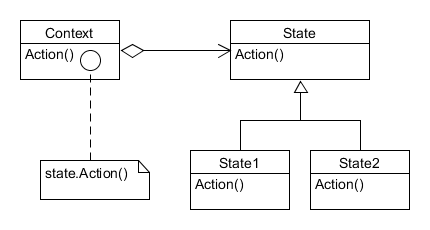
\includegraphics[width=0.7\textwidth]{images/estructura/patrones/state}
	\centering
	\caption{Diagrama de clases del patrón State.}
	\label{state_diagram}
\end{figure}

En el ámbito del videojuego, State se utiliza en la implementación de máquinas de estados, especialmente las dedicadas a la inteligencia artificial. Debido a la aparición de otras técnicas como los \textbf{arboles de comportamiento}, el uso de este patrón no es tan prominente como lo fue en el pasado, pero sigue siendo muy útil en la lectura de entrada, en la navegación de menús o en el procesamiento de textos.
 
En virus breaker, este patrón se utiliza en la implementación del comportamiento del personaje principal, la pelota y el jefe. Esta implementación se realiza mediante plugin \footnote{https://github.com/thefuntastic/Unity3d-Finite-State-Machine} externo. Además, el componente \textbf{Animator} de Unity utiliza una máquina de estados finitos para la gestión de animaciones.

\subsection{Component}
El patrón componente permite a una sola entidad cubrir múltiples dominios sin provocar el acoplamiento entre los distintos dominios cubiertos \cite{game_programming_patterns}.

La forma de implementar este patrón es crear clases \textbf{Componentes} que encapsulan los métodos y atributos que se utilizan para tratar con cierto dominio del programa (como podría ser la entrada del jugador, el sonido o las físicas). Cuando la funcionalidad de una clase afecta a varios dominios del programa, se le asignan los componentes de dichos dominios, en lugar de acceder a los dominios directamente, lo que provocaría un serio acoplamiento del código. Un diagrama con una estructura de clases de ejemplo de este patrón puede verse en la figura \ref{component_diagram}.
\begin{figure}[h]
	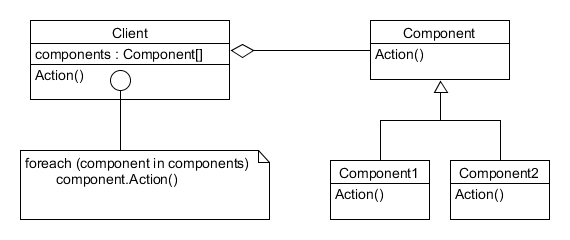
\includegraphics[width=1\textwidth]{images/estructura/patrones/component}
	\centering
	\caption{Diagrama de clases del patrón Component.}
	\label{component_diagram}
\end{figure}

Cuando este patrón se utiliza de forma generalizada en un código, las clases pasan a convertirse en \textbf{contenedores de componentes} cuya funcionalidad se deriva completamente de los componentes que tiene asociados. La única función de estas clases suele ser la de coordinar y gestionar el paso de mensajes entre los distintos componentes.

Actualmente, varios motores de juegos utilizan este patrón en la implementación de entidades del juego, dado que una misma entidad necesita casi siempre controlar varios dominios del programa. Algunos de estos motores son Microsoft XNA \footnote{https://msdn.microsoft.com/es-ES/dn308572} y Unity3D \footnote{https://unity3d.com/es/unity}

\subsection{Prototype}
Este patrón permite especificar tipos de objetos utilizando una \textbf{instancia prototipo} como referencia. Los nuevos objetos se crean realizando copias del prototipo \cite{design_patterns}.

Los prototipos se utilizan para ocultar los detalles de la producción de objetos de una clase a sus usuarios, dotando a las instancias de la capacidad copias de sí mismas, normalmente a través de un método \textbf{clone}. Por ello, este patrón resulta especialmente útil cuando el programa necesita crear diferentes tipos de objetos dependiendo de algún parámetro en tiempo de ejecución o para encapsular procesos de producción de instancias complejos. En el diagrama \ref{prototype_diagram} se puede ver una estructura de clases que ejemplifica este patrón.
\begin{figure}[h]
	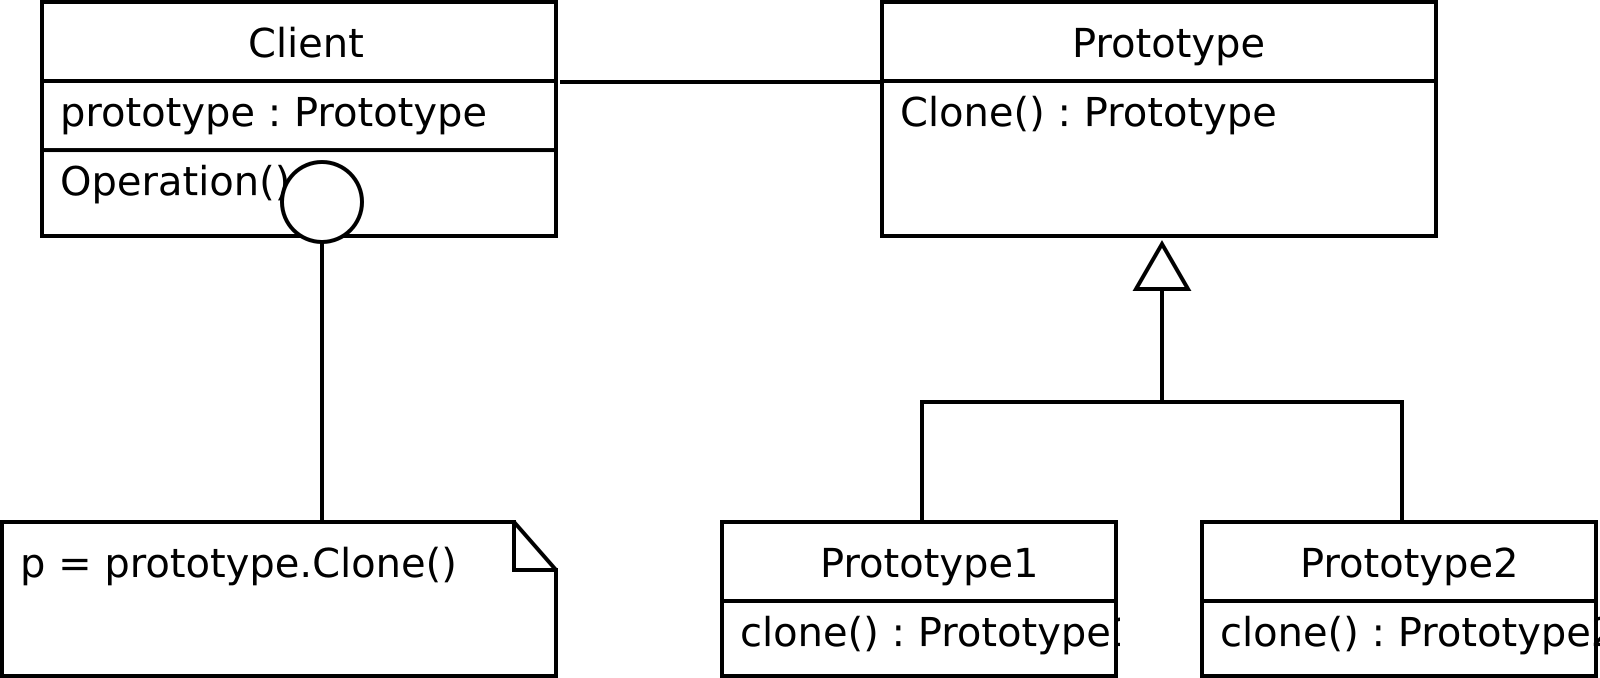
\includegraphics[width=1\textwidth]{images/estructura/patrones/prototype}
	\centering
	\caption{Diagrama de clases del patrón Prototype.}
	\label{prototype_diagram}
\end{figure}

En Unity3D, el patrón Prototype se implementa en su sistema de \textbf{objetos prefabricados}. Este sistema permite guardar los GameObjects creados en el editor a modo como un assets del proyecto de tipo \textbf{Prefab}. Los prefabs pueden ser instanciados desde el editor o en tiempo de ejecución mediante el método estático \textbf{Instantiate}, el cual puede aceptar cualquier GameObject, aunque no se encuentre guardado como prefab. Este sistema simplifica la creación de nuevos GameObjects que, al estar formados por múltiples \textbf{Componentes} asociados, seria desmedidamente engorrosa.

En Virus Breaker, se utilizan prefabricados en múltiples elementos del juego: los ladrillos, la paleta y el jefe son todos objetos prefabricados que se instancian en tiempo de ejecución cuando son necesario. Adicionalmente, otros objetos como la pelota, el jugador y la sala se encuentran guardados como prefabs a modo de copia de seguridad.

\subsection{Singleton}
Este patrón asegura que una clase tenga una sola instancia, y provee acceso global a ella \cite{design_patterns}.

Los singleton se utilizan en sistemas informáticos donde es importante que ciertas clases tengan una única instancia disponible en todo momento. Es útil para sistemas globales a los que deben acceder múltiples objetos, como un sistema de archivos o un gestor de dispositivos externos. Para asegurar la unicidad y accesibilidad de la instancia, el constructor de la clase es privado y en su lugar se utiliza un método estático que da acceso a una instancia de la clase, o la crea en caso de que aún no esté instanciada. La figura \ref{singleton_diagram} muestra el diagrama de la estructura mínima una clase Singleton.
\begin{figure}[h]
	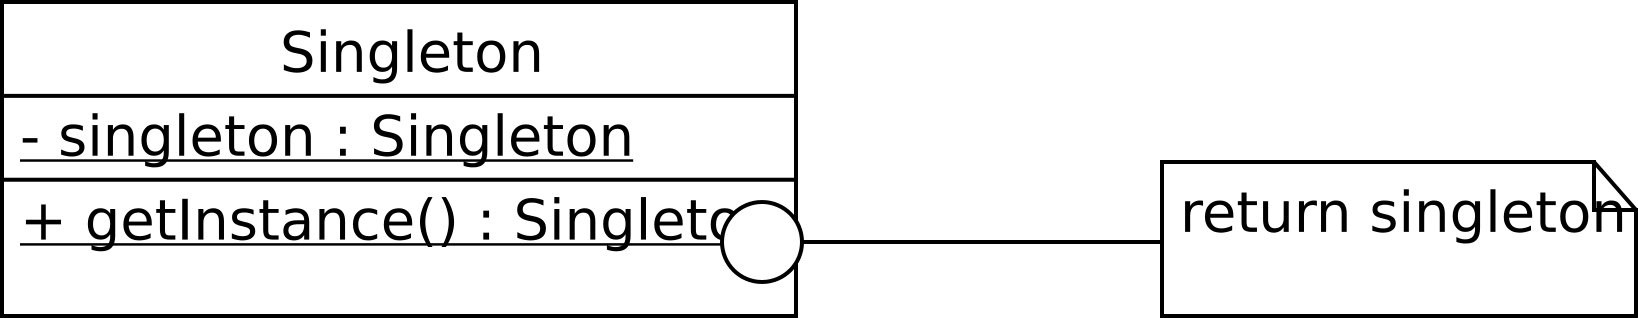
\includegraphics[width=0.7\textwidth]{images/estructura/patrones/singleton}
	\centering
	\caption{Diagrama de clases del patrón Singleton.}
	\label{singleton_diagram}
\end{figure}

El patrón cuenta con mala fama debido a que es común utilizarlo de forma incorrecta, añadiendo más restricciones de las requeridas e introduciendo \textbf{estado global}, que dificulta la depuración del código y aumenta la propensión a errores.

En este proyecto, se utiliza este patrón en la clase \textbf{EscapeController}, el componente que permite salir de la aplicación en cualquier momento pulsando la tecla escape. Al tratarse de un componente, el patrón no puede aplicarse de forma literal por dos motivos:
\begin{enumerate}
\item El \textbf{constructor} de un componente no puede ser modificado ya que interferiría con los sistemas de Unity. En su lugar, en el evento \textbf{Awake} que es invocado al principio de la ejecución revisa si ya existen componentes de esa clase, y lo destruye en caso afirmativo.
\item Al ser un componente, necesita \textbf{estar asignado a un GameObject} para funcionar, los cuales se destruyen por defecto durante los cambios de escena. Para evitarlo, durante la instanciación se llama a la función \textbf{DontDestroyOnLoad} que permite que el objeto persista entre escenas.
\end{enumerate}
